\chapter{Related work and theoretical background}

\section{Related work}

Topological data analysis (TDA) has been applied to neural network research using a wide range of methods.
As outlined in~\cite{ballester2024topologicaldataanalysisneural}, these approaches can be broadly categorized
according to which aspect of neural network they analyze:
\begin{enumerate}
    \item \emph{Structure of neural networks}, such as in~\cite{Chowdhury_2019},
    where two special homology groups are computed for graphs that represent feed-forward neural networks.
    \item \emph{Decision regions and boundaries}. In~\cite{ramamurthy2018topologicaldataanalysisdecision},
    the labeled \v{C}ech and Vietoris-Rips complexes are introduced to capture homology of neural network decision boundaries.
    This approach is augmented with active learning in~\cite{NEURIPS2020_5f146156} to improve sampling efficiency.
    Several other studies employ the \emph{graph-based topological data analysis} (GTDA) algorithm~\cite{Liu2023},
    an extension of the Mapper algorithm~\cite{:10.2312/SPBG/SPBG07/091-100} that handles graph inputs and generates Reeb networks.
    \label{item:decision}
    \item \emph{Activations and weights}.
    Methods in this category apply either the Mapper algorithm~\cite{8999218,love2020topological,9174770},
    or persistent homology~\cite{8953424,gebhart2019characterizingshapeactivationspace,https://doi.org/10.3929/ethz-b-000327207}
    to neural network weights or activations.
    \item \emph{Training dynamics and loss functions}.
    In~\cite{nguyen2019connectedsublevelsetsdeep} the number of connected components and local valleys
    of a convex optimization target are studied in the context of fully connected feed-forward neural networks.
    In~\cite{_im_ekli_2021} and~\cite{birdal2021intrinsicdimensionpersistenthomology},
    the fractal dimensions of weight trajectories of neural networks during training are studied.
    \label{item:training}
\end{enumerate}

This research bridges the categories~\ref{item:decision} and~\ref{item:training},
presenting a novel investigation that combines topological analysis of decision boundaries
with neural network training dynamics.

\section{Theoretical background}

\subsection{Persistent homology}

Persistent homology serves as a fundamental tool in TDA that tracks how topological
features (connected components, holes) appear and disappear as a parameter is varied.
Given a filtered simplicial complex $(K_\epsilon)_{\epsilon \geq 0}$, persistent homology computes pairs
$(\epsilon_b, \epsilon_d)$ where a feature appears at $\epsilon_b$ (birth) and
disappears at $\epsilon_d$ (death).

These birth--death pairs can be visualized in a \emph{persistence diagram}, where each pair
is shown as a point in the Euclidean plane. The distance of a point from the diagonal
indicates the feature's persistence, which is often interpreted as a measure of
its significance. Figure~\ref{fig:pd} shows an example of a persistence diagram.

\begin{figure}
    \centering
    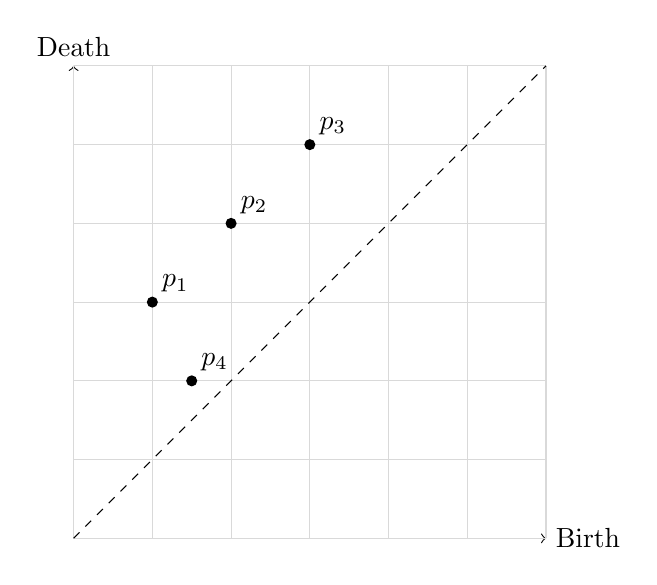
\begin{tikzpicture}
        % Axes
        \draw[->] (0,0) -- (6,0) node[right] {Birth};
        \draw[->] (0,0) -- (0,6) node[above] {Death};
        
        % Grid
        \draw[gray!30] (0,0) grid (6,6);
        
        % Diagonal
        \draw[dashed] (0,0) -- (6,6);
        
        % Points
        \fill (1,3) circle (2pt) node[above right] {$p_1$};
        \fill (2,4) circle (2pt) node[above right] {$p_2$};
        \fill (3,5) circle (2pt) node[above right] {$p_3$};
        \fill (1.5,2) circle (2pt) node[above right] {$p_4$};
    \end{tikzpicture}
    \caption{An example of a persistent diagram.}
    \label{fig:pd}
\end{figure}

\subsection{Labeled \v{C}ech complex}

\begin{definition}[Labeled \v{C}ech (L\v{C}) complex, \cite{ramamurthy2018topologicaldataanalysisdecision}]
    Given a set of points \(X\), a reference set \(Y\), and parameters \(\varepsilon\) and \(\gamma\),
    the \emph{labeled \v{C}ech complex} contains
    an \(n\)-simplex formed by points \(x_0, \dots, x_n \in X\) if and only if:
    \begin{enumerate}
        \item \(\bigcap_{i = 0}^n B_\varepsilon(x_i) \neq \emptyset\)
        \item For each \(i \in (0, \dots, n)\), there exists \(y \in Y\) such that
        \(\norm{x_i - y} \leq \gamma\).
    \end{enumerate}
    This simplicial complex is denoted as \(L\check{C}_{X, Y}^{\varepsilon, \gamma}\).
\end{definition}
In~\cite{ramamurthy2018topologicaldataanalysisdecision}, the \emph{labeled \v{C}ech filtration}
is obtained by varying \(\varepsilon\), while keeping \(\gamma\) fixed.

In binary classification, \(X\) is set of points
of one class, while \(Y\) is set of points of the other class.
Then, \(L\check{C}\) captures simplices on one side of the boundary.
This can be seen in Figure~\ref{fig:lc}.

\begin{figure}
    \centering
    \resizebox{0.8\textwidth}{!}{%% Creator: Matplotlib, PGF backend
%%
%% To include the figure in your LaTeX document, write
%%   \input{<filename>.pgf}
%%
%% Make sure the required packages are loaded in your preamble
%%   \usepackage{pgf}
%%
%% Also ensure that all the required font packages are loaded; for instance,
%% the lmodern package is sometimes necessary when using math font.
%%   \usepackage{lmodern}
%%
%% Figures using additional raster images can only be included by \input if
%% they are in the same directory as the main LaTeX file. For loading figures
%% from other directories you can use the `import` package
%%   \usepackage{import}
%%
%% and then include the figures with
%%   \import{<path to file>}{<filename>.pgf}
%%
%% Matplotlib used the following preamble
%%   \def\mathdefault#1{#1}
%%   \everymath=\expandafter{\the\everymath\displaystyle}
%%   \IfFileExists{scrextend.sty}{
%%     \usepackage[fontsize=10.000000pt]{scrextend}
%%   }{
%%     \renewcommand{\normalsize}{\fontsize{10.000000}{12.000000}\selectfont}
%%     \normalsize
%%   }
%%   
%%   \ifdefined\pdftexversion\else  % non-pdftex case.
%%     \usepackage{fontspec}
%%     \setmainfont{DejaVuSerif.ttf}[Path=\detokenize{/home/snek/repos/semester-project-thesis/venv/lib/python3.13/site-packages/matplotlib/mpl-data/fonts/ttf/}]
%%     \setsansfont{DejaVuSans.ttf}[Path=\detokenize{/home/snek/repos/semester-project-thesis/venv/lib/python3.13/site-packages/matplotlib/mpl-data/fonts/ttf/}]
%%     \setmonofont{DejaVuSansMono.ttf}[Path=\detokenize{/home/snek/repos/semester-project-thesis/venv/lib/python3.13/site-packages/matplotlib/mpl-data/fonts/ttf/}]
%%   \fi
%%   \makeatletter\@ifpackageloaded{underscore}{}{\usepackage[strings]{underscore}}\makeatother
%%
\begingroup%
\makeatletter%
\begin{pgfpicture}%
\pgfpathrectangle{\pgfpointorigin}{\pgfqpoint{6.400000in}{4.800000in}}%
\pgfusepath{use as bounding box, clip}%
\begin{pgfscope}%
\pgfsetbuttcap%
\pgfsetmiterjoin%
\definecolor{currentfill}{rgb}{1.000000,1.000000,1.000000}%
\pgfsetfillcolor{currentfill}%
\pgfsetlinewidth{0.000000pt}%
\definecolor{currentstroke}{rgb}{1.000000,1.000000,1.000000}%
\pgfsetstrokecolor{currentstroke}%
\pgfsetdash{}{0pt}%
\pgfpathmoveto{\pgfqpoint{0.000000in}{0.000000in}}%
\pgfpathlineto{\pgfqpoint{6.400000in}{0.000000in}}%
\pgfpathlineto{\pgfqpoint{6.400000in}{4.800000in}}%
\pgfpathlineto{\pgfqpoint{0.000000in}{4.800000in}}%
\pgfpathlineto{\pgfqpoint{0.000000in}{0.000000in}}%
\pgfpathclose%
\pgfusepath{fill}%
\end{pgfscope}%
\begin{pgfscope}%
\pgfpathrectangle{\pgfqpoint{0.150000in}{0.152203in}}{\pgfqpoint{6.100000in}{4.495594in}}%
\pgfusepath{clip}%
\pgfsetbuttcap%
\pgfsetmiterjoin%
\definecolor{currentfill}{rgb}{0.501961,0.501961,0.501961}%
\pgfsetfillcolor{currentfill}%
\pgfsetfillopacity{0.300000}%
\pgfsetlinewidth{1.003750pt}%
\definecolor{currentstroke}{rgb}{0.501961,0.501961,0.501961}%
\pgfsetstrokecolor{currentstroke}%
\pgfsetdash{}{0pt}%
\pgfpathmoveto{\pgfqpoint{2.367416in}{0.934761in}}%
\pgfpathlineto{\pgfqpoint{2.332158in}{0.924419in}}%
\pgfpathlineto{\pgfqpoint{2.296382in}{0.916039in}}%
\pgfpathlineto{\pgfqpoint{2.260199in}{0.909646in}}%
\pgfpathlineto{\pgfqpoint{2.223718in}{0.905260in}}%
\pgfpathlineto{\pgfqpoint{2.187050in}{0.902895in}}%
\pgfpathlineto{\pgfqpoint{2.150308in}{0.902556in}}%
\pgfpathlineto{\pgfqpoint{2.113603in}{0.904247in}}%
\pgfpathlineto{\pgfqpoint{2.077047in}{0.907960in}}%
\pgfpathlineto{\pgfqpoint{2.040752in}{0.913686in}}%
\pgfpathlineto{\pgfqpoint{2.004828in}{0.921406in}}%
\pgfpathlineto{\pgfqpoint{1.969385in}{0.931098in}}%
\pgfpathlineto{\pgfqpoint{1.934531in}{0.942731in}}%
\pgfpathlineto{\pgfqpoint{1.900373in}{0.956270in}}%
\pgfpathlineto{\pgfqpoint{1.867013in}{0.971673in}}%
\pgfpathlineto{\pgfqpoint{1.834555in}{0.988895in}}%
\pgfpathlineto{\pgfqpoint{1.803097in}{1.007882in}}%
\pgfpathlineto{\pgfqpoint{1.783910in}{1.019174in}}%
\pgfpathlineto{\pgfqpoint{1.747615in}{1.024900in}}%
\pgfpathlineto{\pgfqpoint{1.711691in}{1.032620in}}%
\pgfpathlineto{\pgfqpoint{1.676249in}{1.042312in}}%
\pgfpathlineto{\pgfqpoint{1.641395in}{1.053944in}}%
\pgfpathlineto{\pgfqpoint{1.607236in}{1.067483in}}%
\pgfpathlineto{\pgfqpoint{1.573877in}{1.082887in}}%
\pgfpathlineto{\pgfqpoint{1.558094in}{1.090354in}}%
\pgfpathlineto{\pgfqpoint{1.521351in}{1.090692in}}%
\pgfpathlineto{\pgfqpoint{1.484684in}{1.093058in}}%
\pgfpathlineto{\pgfqpoint{1.448202in}{1.097444in}}%
\pgfpathlineto{\pgfqpoint{1.412019in}{1.103837in}}%
\pgfpathlineto{\pgfqpoint{1.376243in}{1.112217in}}%
\pgfpathlineto{\pgfqpoint{1.340985in}{1.122559in}}%
\pgfpathlineto{\pgfqpoint{1.306351in}{1.134831in}}%
\pgfpathlineto{\pgfqpoint{1.272447in}{1.148997in}}%
\pgfpathlineto{\pgfqpoint{1.239377in}{1.165012in}}%
\pgfpathlineto{\pgfqpoint{1.207241in}{1.182828in}}%
\pgfpathlineto{\pgfqpoint{1.176138in}{1.202391in}}%
\pgfpathlineto{\pgfqpoint{1.146162in}{1.223640in}}%
\pgfpathlineto{\pgfqpoint{1.117404in}{1.246512in}}%
\pgfpathlineto{\pgfqpoint{1.089953in}{1.270936in}}%
\pgfpathlineto{\pgfqpoint{1.063891in}{1.296838in}}%
\pgfpathlineto{\pgfqpoint{1.039299in}{1.324139in}}%
\pgfpathlineto{\pgfqpoint{1.016251in}{1.352756in}}%
\pgfpathlineto{\pgfqpoint{0.994818in}{1.382601in}}%
\pgfpathlineto{\pgfqpoint{0.975065in}{1.413584in}}%
\pgfpathlineto{\pgfqpoint{0.957053in}{1.445610in}}%
\pgfpathlineto{\pgfqpoint{0.940835in}{1.478581in}}%
\pgfpathlineto{\pgfqpoint{0.926462in}{1.512397in}}%
\pgfpathlineto{\pgfqpoint{0.913977in}{1.546955in}}%
\pgfpathlineto{\pgfqpoint{0.903419in}{1.582149in}}%
\pgfpathlineto{\pgfqpoint{0.894819in}{1.617873in}}%
\pgfpathlineto{\pgfqpoint{0.888204in}{1.654016in}}%
\pgfpathlineto{\pgfqpoint{0.883997in}{1.680246in}}%
\pgfpathlineto{\pgfqpoint{0.867982in}{1.713316in}}%
\pgfpathlineto{\pgfqpoint{0.853817in}{1.747219in}}%
\pgfpathlineto{\pgfqpoint{0.841544in}{1.781853in}}%
\pgfpathlineto{\pgfqpoint{0.831202in}{1.817112in}}%
\pgfpathlineto{\pgfqpoint{0.822822in}{1.852887in}}%
\pgfpathlineto{\pgfqpoint{0.816429in}{1.889071in}}%
\pgfpathlineto{\pgfqpoint{0.813027in}{1.910480in}}%
\pgfpathlineto{\pgfqpoint{0.788102in}{1.937477in}}%
\pgfpathlineto{\pgfqpoint{0.764705in}{1.965809in}}%
\pgfpathlineto{\pgfqpoint{0.742907in}{1.995389in}}%
\pgfpathlineto{\pgfqpoint{0.722775in}{2.026127in}}%
\pgfpathlineto{\pgfqpoint{0.704371in}{2.057930in}}%
\pgfpathlineto{\pgfqpoint{0.687750in}{2.090699in}}%
\pgfpathlineto{\pgfqpoint{0.672963in}{2.124336in}}%
\pgfpathlineto{\pgfqpoint{0.660055in}{2.158739in}}%
\pgfpathlineto{\pgfqpoint{0.649066in}{2.193801in}}%
\pgfpathlineto{\pgfqpoint{0.640028in}{2.229416in}}%
\pgfpathlineto{\pgfqpoint{0.632970in}{2.265476in}}%
\pgfpathlineto{\pgfqpoint{0.627914in}{2.301870in}}%
\pgfpathlineto{\pgfqpoint{0.624873in}{2.338488in}}%
\pgfpathlineto{\pgfqpoint{0.623859in}{2.375218in}}%
\pgfpathlineto{\pgfqpoint{0.624873in}{2.411948in}}%
\pgfpathlineto{\pgfqpoint{0.627914in}{2.448566in}}%
\pgfpathlineto{\pgfqpoint{0.632970in}{2.484960in}}%
\pgfpathlineto{\pgfqpoint{0.640028in}{2.521020in}}%
\pgfpathlineto{\pgfqpoint{0.649066in}{2.556635in}}%
\pgfpathlineto{\pgfqpoint{0.660055in}{2.591697in}}%
\pgfpathlineto{\pgfqpoint{0.672963in}{2.626099in}}%
\pgfpathlineto{\pgfqpoint{0.687750in}{2.659736in}}%
\pgfpathlineto{\pgfqpoint{0.704371in}{2.692506in}}%
\pgfpathlineto{\pgfqpoint{0.722775in}{2.724308in}}%
\pgfpathlineto{\pgfqpoint{0.742907in}{2.755046in}}%
\pgfpathlineto{\pgfqpoint{0.764705in}{2.784626in}}%
\pgfpathlineto{\pgfqpoint{0.788102in}{2.812958in}}%
\pgfpathlineto{\pgfqpoint{0.813027in}{2.839955in}}%
\pgfpathlineto{\pgfqpoint{0.839405in}{2.865536in}}%
\pgfpathlineto{\pgfqpoint{0.867154in}{2.889621in}}%
\pgfpathlineto{\pgfqpoint{0.896190in}{2.912138in}}%
\pgfpathlineto{\pgfqpoint{0.926425in}{2.933018in}}%
\pgfpathlineto{\pgfqpoint{0.957766in}{2.952198in}}%
\pgfpathlineto{\pgfqpoint{0.990118in}{2.969618in}}%
\pgfpathlineto{\pgfqpoint{1.023382in}{2.985226in}}%
\pgfpathlineto{\pgfqpoint{1.057457in}{2.998974in}}%
\pgfpathlineto{\pgfqpoint{1.092239in}{3.010821in}}%
\pgfpathlineto{\pgfqpoint{1.127621in}{3.020729in}}%
\pgfpathlineto{\pgfqpoint{1.163497in}{3.028670in}}%
\pgfpathlineto{\pgfqpoint{1.199756in}{3.034618in}}%
\pgfpathlineto{\pgfqpoint{1.236289in}{3.038556in}}%
\pgfpathlineto{\pgfqpoint{1.272983in}{3.040472in}}%
\pgfpathlineto{\pgfqpoint{1.309726in}{3.040359in}}%
\pgfpathlineto{\pgfqpoint{1.346408in}{3.038218in}}%
\pgfpathlineto{\pgfqpoint{1.382915in}{3.034056in}}%
\pgfpathlineto{\pgfqpoint{1.419137in}{3.027886in}}%
\pgfpathlineto{\pgfqpoint{1.454964in}{3.019725in}}%
\pgfpathlineto{\pgfqpoint{1.485826in}{3.012574in}}%
\pgfpathlineto{\pgfqpoint{1.514443in}{3.035622in}}%
\pgfpathlineto{\pgfqpoint{1.544288in}{3.057055in}}%
\pgfpathlineto{\pgfqpoint{1.573787in}{3.075912in}}%
\pgfpathlineto{\pgfqpoint{1.567309in}{3.110346in}}%
\pgfpathlineto{\pgfqpoint{1.562476in}{3.146771in}}%
\pgfpathlineto{\pgfqpoint{1.559660in}{3.183407in}}%
\pgfpathlineto{\pgfqpoint{1.558871in}{3.220142in}}%
\pgfpathlineto{\pgfqpoint{1.560111in}{3.256865in}}%
\pgfpathlineto{\pgfqpoint{1.563376in}{3.293464in}}%
\pgfpathlineto{\pgfqpoint{1.568656in}{3.329826in}}%
\pgfpathlineto{\pgfqpoint{1.575935in}{3.365842in}}%
\pgfpathlineto{\pgfqpoint{1.585190in}{3.401401in}}%
\pgfpathlineto{\pgfqpoint{1.596395in}{3.436395in}}%
\pgfpathlineto{\pgfqpoint{1.611835in}{3.483183in}}%
\pgfpathlineto{\pgfqpoint{1.620434in}{3.518906in}}%
\pgfpathlineto{\pgfqpoint{1.630993in}{3.554100in}}%
\pgfpathlineto{\pgfqpoint{1.643477in}{3.588658in}}%
\pgfpathlineto{\pgfqpoint{1.657851in}{3.622474in}}%
\pgfpathlineto{\pgfqpoint{1.674068in}{3.655446in}}%
\pgfpathlineto{\pgfqpoint{1.692081in}{3.687471in}}%
\pgfpathlineto{\pgfqpoint{1.711834in}{3.718454in}}%
\pgfpathlineto{\pgfqpoint{1.733267in}{3.748299in}}%
\pgfpathlineto{\pgfqpoint{1.756315in}{3.776916in}}%
\pgfpathlineto{\pgfqpoint{1.780907in}{3.804217in}}%
\pgfpathlineto{\pgfqpoint{1.806969in}{3.830119in}}%
\pgfpathlineto{\pgfqpoint{1.834420in}{3.854543in}}%
\pgfpathlineto{\pgfqpoint{1.863178in}{3.877415in}}%
\pgfpathlineto{\pgfqpoint{1.893154in}{3.898665in}}%
\pgfpathlineto{\pgfqpoint{1.924257in}{3.918227in}}%
\pgfpathlineto{\pgfqpoint{1.956393in}{3.936043in}}%
\pgfpathlineto{\pgfqpoint{1.989463in}{3.952058in}}%
\pgfpathlineto{\pgfqpoint{2.023367in}{3.966224in}}%
\pgfpathlineto{\pgfqpoint{2.058001in}{3.978496in}}%
\pgfpathlineto{\pgfqpoint{2.093259in}{3.988838in}}%
\pgfpathlineto{\pgfqpoint{2.129035in}{3.997219in}}%
\pgfpathlineto{\pgfqpoint{2.165218in}{4.003611in}}%
\pgfpathlineto{\pgfqpoint{2.201699in}{4.007997in}}%
\pgfpathlineto{\pgfqpoint{2.238367in}{4.010363in}}%
\pgfpathlineto{\pgfqpoint{2.275109in}{4.010701in}}%
\pgfpathlineto{\pgfqpoint{2.311814in}{4.009011in}}%
\pgfpathlineto{\pgfqpoint{2.348370in}{4.005297in}}%
\pgfpathlineto{\pgfqpoint{2.384665in}{3.999571in}}%
\pgfpathlineto{\pgfqpoint{2.420589in}{3.991851in}}%
\pgfpathlineto{\pgfqpoint{2.456032in}{3.982160in}}%
\pgfpathlineto{\pgfqpoint{2.490886in}{3.970527in}}%
\pgfpathlineto{\pgfqpoint{2.525044in}{3.956988in}}%
\pgfpathlineto{\pgfqpoint{2.604144in}{3.921777in}}%
\pgfpathlineto{\pgfqpoint{2.636388in}{3.904159in}}%
\pgfpathlineto{\pgfqpoint{2.667611in}{3.884787in}}%
\pgfpathlineto{\pgfqpoint{2.697717in}{3.863722in}}%
\pgfpathlineto{\pgfqpoint{2.726615in}{3.841027in}}%
\pgfpathlineto{\pgfqpoint{2.754215in}{3.816772in}}%
\pgfpathlineto{\pgfqpoint{2.780435in}{3.791031in}}%
\pgfpathlineto{\pgfqpoint{2.805194in}{3.763881in}}%
\pgfpathlineto{\pgfqpoint{2.828417in}{3.735406in}}%
\pgfpathlineto{\pgfqpoint{2.850033in}{3.705693in}}%
\pgfpathlineto{\pgfqpoint{2.869976in}{3.674832in}}%
\pgfpathlineto{\pgfqpoint{2.888185in}{3.642917in}}%
\pgfpathlineto{\pgfqpoint{2.904605in}{3.610046in}}%
\pgfpathlineto{\pgfqpoint{2.919185in}{3.576319in}}%
\pgfpathlineto{\pgfqpoint{2.931881in}{3.541838in}}%
\pgfpathlineto{\pgfqpoint{2.942655in}{3.506709in}}%
\pgfpathlineto{\pgfqpoint{2.951474in}{3.471039in}}%
\pgfpathlineto{\pgfqpoint{2.955157in}{3.452939in}}%
\pgfpathlineto{\pgfqpoint{2.982997in}{3.430486in}}%
\pgfpathlineto{\pgfqpoint{3.010298in}{3.405894in}}%
\pgfpathlineto{\pgfqpoint{3.036200in}{3.379832in}}%
\pgfpathlineto{\pgfqpoint{3.060624in}{3.352381in}}%
\pgfpathlineto{\pgfqpoint{3.083496in}{3.323623in}}%
\pgfpathlineto{\pgfqpoint{3.103976in}{3.294791in}}%
\pgfpathlineto{\pgfqpoint{3.136552in}{3.308363in}}%
\pgfpathlineto{\pgfqpoint{3.171186in}{3.320635in}}%
\pgfpathlineto{\pgfqpoint{3.206444in}{3.330977in}}%
\pgfpathlineto{\pgfqpoint{3.242220in}{3.339358in}}%
\pgfpathlineto{\pgfqpoint{3.278403in}{3.345750in}}%
\pgfpathlineto{\pgfqpoint{3.314885in}{3.350136in}}%
\pgfpathlineto{\pgfqpoint{3.351552in}{3.352502in}}%
\pgfpathlineto{\pgfqpoint{3.388295in}{3.352840in}}%
\pgfpathlineto{\pgfqpoint{3.425000in}{3.351150in}}%
\pgfpathlineto{\pgfqpoint{3.461555in}{3.347436in}}%
\pgfpathlineto{\pgfqpoint{3.497851in}{3.341710in}}%
\pgfpathlineto{\pgfqpoint{3.533774in}{3.333990in}}%
\pgfpathlineto{\pgfqpoint{3.569217in}{3.324299in}}%
\pgfpathlineto{\pgfqpoint{3.604071in}{3.312666in}}%
\pgfpathlineto{\pgfqpoint{3.638230in}{3.299127in}}%
\pgfpathlineto{\pgfqpoint{3.671589in}{3.283723in}}%
\pgfpathlineto{\pgfqpoint{3.704047in}{3.266502in}}%
\pgfpathlineto{\pgfqpoint{3.735505in}{3.247515in}}%
\pgfpathlineto{\pgfqpoint{3.765868in}{3.226821in}}%
\pgfpathlineto{\pgfqpoint{3.795041in}{3.204482in}}%
\pgfpathlineto{\pgfqpoint{3.822938in}{3.180568in}}%
\pgfpathlineto{\pgfqpoint{3.849472in}{3.155150in}}%
\pgfpathlineto{\pgfqpoint{3.874562in}{3.128306in}}%
\pgfpathlineto{\pgfqpoint{3.898133in}{3.100118in}}%
\pgfpathlineto{\pgfqpoint{3.920111in}{3.070673in}}%
\pgfpathlineto{\pgfqpoint{3.940431in}{3.040059in}}%
\pgfpathlineto{\pgfqpoint{3.959031in}{3.008370in}}%
\pgfpathlineto{\pgfqpoint{3.975852in}{2.975703in}}%
\pgfpathlineto{\pgfqpoint{3.990846in}{2.942157in}}%
\pgfpathlineto{\pgfqpoint{4.003964in}{2.907835in}}%
\pgfpathlineto{\pgfqpoint{4.015169in}{2.872841in}}%
\pgfpathlineto{\pgfqpoint{4.024424in}{2.837282in}}%
\pgfpathlineto{\pgfqpoint{4.031703in}{2.801266in}}%
\pgfpathlineto{\pgfqpoint{4.036983in}{2.764903in}}%
\pgfpathlineto{\pgfqpoint{4.040248in}{2.728305in}}%
\pgfpathlineto{\pgfqpoint{4.041488in}{2.691582in}}%
\pgfpathlineto{\pgfqpoint{4.040699in}{2.654846in}}%
\pgfpathlineto{\pgfqpoint{4.037883in}{2.618210in}}%
\pgfpathlineto{\pgfqpoint{4.036032in}{2.597620in}}%
\pgfpathlineto{\pgfqpoint{4.046374in}{2.562362in}}%
\pgfpathlineto{\pgfqpoint{4.054754in}{2.526586in}}%
\pgfpathlineto{\pgfqpoint{4.061147in}{2.490403in}}%
\pgfpathlineto{\pgfqpoint{4.065533in}{2.453921in}}%
\pgfpathlineto{\pgfqpoint{4.067899in}{2.417254in}}%
\pgfpathlineto{\pgfqpoint{4.068237in}{2.380511in}}%
\pgfpathlineto{\pgfqpoint{4.066546in}{2.343806in}}%
\pgfpathlineto{\pgfqpoint{4.062833in}{2.307251in}}%
\pgfpathlineto{\pgfqpoint{4.057107in}{2.270956in}}%
\pgfpathlineto{\pgfqpoint{4.049387in}{2.235032in}}%
\pgfpathlineto{\pgfqpoint{4.039695in}{2.199589in}}%
\pgfpathlineto{\pgfqpoint{4.028062in}{2.164735in}}%
\pgfpathlineto{\pgfqpoint{4.014523in}{2.130576in}}%
\pgfpathlineto{\pgfqpoint{4.011808in}{2.123537in}}%
\pgfpathlineto{\pgfqpoint{4.017534in}{2.087242in}}%
\pgfpathlineto{\pgfqpoint{4.021247in}{2.050686in}}%
\pgfpathlineto{\pgfqpoint{4.022938in}{2.013981in}}%
\pgfpathlineto{\pgfqpoint{4.022599in}{1.977238in}}%
\pgfpathlineto{\pgfqpoint{4.020234in}{1.940571in}}%
\pgfpathlineto{\pgfqpoint{4.015848in}{1.904089in}}%
\pgfpathlineto{\pgfqpoint{4.009455in}{1.867906in}}%
\pgfpathlineto{\pgfqpoint{4.001075in}{1.832130in}}%
\pgfpathlineto{\pgfqpoint{3.990733in}{1.796872in}}%
\pgfpathlineto{\pgfqpoint{3.978460in}{1.762238in}}%
\pgfpathlineto{\pgfqpoint{3.964295in}{1.728334in}}%
\pgfpathlineto{\pgfqpoint{3.948280in}{1.695264in}}%
\pgfpathlineto{\pgfqpoint{3.930464in}{1.663129in}}%
\pgfpathlineto{\pgfqpoint{3.910901in}{1.632025in}}%
\pgfpathlineto{\pgfqpoint{3.889652in}{1.602049in}}%
\pgfpathlineto{\pgfqpoint{3.866780in}{1.573291in}}%
\pgfpathlineto{\pgfqpoint{3.842356in}{1.545840in}}%
\pgfpathlineto{\pgfqpoint{3.816454in}{1.519778in}}%
\pgfpathlineto{\pgfqpoint{3.789153in}{1.495186in}}%
\pgfpathlineto{\pgfqpoint{3.760536in}{1.472139in}}%
\pgfpathlineto{\pgfqpoint{3.730691in}{1.450706in}}%
\pgfpathlineto{\pgfqpoint{3.699708in}{1.430952in}}%
\pgfpathlineto{\pgfqpoint{3.667682in}{1.412940in}}%
\pgfpathlineto{\pgfqpoint{3.634711in}{1.396722in}}%
\pgfpathlineto{\pgfqpoint{3.600895in}{1.382349in}}%
\pgfpathlineto{\pgfqpoint{3.566337in}{1.369864in}}%
\pgfpathlineto{\pgfqpoint{3.538216in}{1.359903in}}%
\pgfpathlineto{\pgfqpoint{3.533606in}{1.323450in}}%
\pgfpathlineto{\pgfqpoint{3.526991in}{1.287306in}}%
\pgfpathlineto{\pgfqpoint{3.518392in}{1.251583in}}%
\pgfpathlineto{\pgfqpoint{3.507833in}{1.216388in}}%
\pgfpathlineto{\pgfqpoint{3.495349in}{1.181831in}}%
\pgfpathlineto{\pgfqpoint{3.480976in}{1.148014in}}%
\pgfpathlineto{\pgfqpoint{3.464758in}{1.115043in}}%
\pgfpathlineto{\pgfqpoint{3.446745in}{1.083017in}}%
\pgfpathlineto{\pgfqpoint{3.426992in}{1.052035in}}%
\pgfpathlineto{\pgfqpoint{3.405559in}{1.022189in}}%
\pgfpathlineto{\pgfqpoint{3.382511in}{0.993573in}}%
\pgfpathlineto{\pgfqpoint{3.357919in}{0.966272in}}%
\pgfpathlineto{\pgfqpoint{3.331858in}{0.940369in}}%
\pgfpathlineto{\pgfqpoint{3.304406in}{0.915945in}}%
\pgfpathlineto{\pgfqpoint{3.275649in}{0.893074in}}%
\pgfpathlineto{\pgfqpoint{3.245672in}{0.871824in}}%
\pgfpathlineto{\pgfqpoint{3.214569in}{0.852262in}}%
\pgfpathlineto{\pgfqpoint{3.182433in}{0.834446in}}%
\pgfpathlineto{\pgfqpoint{3.149363in}{0.818431in}}%
\pgfpathlineto{\pgfqpoint{3.115459in}{0.804265in}}%
\pgfpathlineto{\pgfqpoint{3.080826in}{0.791993in}}%
\pgfpathlineto{\pgfqpoint{3.045567in}{0.781651in}}%
\pgfpathlineto{\pgfqpoint{3.009792in}{0.773270in}}%
\pgfpathlineto{\pgfqpoint{2.973608in}{0.766877in}}%
\pgfpathlineto{\pgfqpoint{2.937127in}{0.762491in}}%
\pgfpathlineto{\pgfqpoint{2.900459in}{0.760126in}}%
\pgfpathlineto{\pgfqpoint{2.863717in}{0.759788in}}%
\pgfpathlineto{\pgfqpoint{2.827012in}{0.761478in}}%
\pgfpathlineto{\pgfqpoint{2.790456in}{0.765192in}}%
\pgfpathlineto{\pgfqpoint{2.754161in}{0.770917in}}%
\pgfpathlineto{\pgfqpoint{2.718237in}{0.778638in}}%
\pgfpathlineto{\pgfqpoint{2.682794in}{0.788329in}}%
\pgfpathlineto{\pgfqpoint{2.647940in}{0.799962in}}%
\pgfpathlineto{\pgfqpoint{2.613782in}{0.813501in}}%
\pgfpathlineto{\pgfqpoint{2.580422in}{0.828905in}}%
\pgfpathlineto{\pgfqpoint{2.547964in}{0.846126in}}%
\pgfpathlineto{\pgfqpoint{2.516506in}{0.865113in}}%
\pgfpathlineto{\pgfqpoint{2.486144in}{0.885807in}}%
\pgfpathlineto{\pgfqpoint{2.456970in}{0.908145in}}%
\pgfpathlineto{\pgfqpoint{2.447151in}{0.915400in}}%
\pgfpathlineto{\pgfqpoint{2.410769in}{0.931425in}}%
\pgfpathlineto{\pgfqpoint{2.367416in}{0.934761in}}%
\pgfpathlineto{\pgfqpoint{2.367416in}{0.934761in}}%
\pgfusepath{stroke,fill}%
\end{pgfscope}%
\begin{pgfscope}%
\pgfpathrectangle{\pgfqpoint{0.150000in}{0.152203in}}{\pgfqpoint{6.100000in}{4.495594in}}%
\pgfusepath{clip}%
\pgfsetbuttcap%
\pgfsetroundjoin%
\definecolor{currentfill}{rgb}{0.121569,0.466667,0.705882}%
\pgfsetfillcolor{currentfill}%
\pgfsetlinewidth{1.003750pt}%
\definecolor{currentstroke}{rgb}{0.121569,0.466667,0.705882}%
\pgfsetstrokecolor{currentstroke}%
\pgfsetdash{}{0pt}%
\pgfsys@defobject{currentmarker}{\pgfqpoint{-0.041667in}{-0.041667in}}{\pgfqpoint{0.041667in}{0.041667in}}{%
\pgfpathmoveto{\pgfqpoint{0.000000in}{0.041667in}}%
\pgfpathlineto{\pgfqpoint{-0.041667in}{-0.041667in}}%
\pgfpathlineto{\pgfqpoint{0.041667in}{-0.041667in}}%
\pgfpathlineto{\pgfqpoint{0.000000in}{0.041667in}}%
\pgfpathclose%
\pgfusepath{stroke,fill}%
}%
\begin{pgfscope}%
\pgfsys@transformshift{3.255455in}{3.225376in}%
\pgfsys@useobject{currentmarker}{}%
\end{pgfscope}%
\begin{pgfscope}%
\pgfsys@transformshift{3.701367in}{2.779143in}%
\pgfsys@useobject{currentmarker}{}%
\end{pgfscope}%
\begin{pgfscope}%
\pgfsys@transformshift{3.410901in}{2.811250in}%
\pgfsys@useobject{currentmarker}{}%
\end{pgfscope}%
\begin{pgfscope}%
\pgfsys@transformshift{3.523417in}{3.018819in}%
\pgfsys@useobject{currentmarker}{}%
\end{pgfscope}%
\begin{pgfscope}%
\pgfsys@transformshift{2.338138in}{3.466307in}%
\pgfsys@useobject{currentmarker}{}%
\end{pgfscope}%
\begin{pgfscope}%
\pgfsys@transformshift{1.648837in}{3.487781in}%
\pgfsys@useobject{currentmarker}{}%
\end{pgfscope}%
\begin{pgfscope}%
\pgfsys@transformshift{1.652603in}{3.249547in}%
\pgfsys@useobject{currentmarker}{}%
\end{pgfscope}%
\begin{pgfscope}%
\pgfsys@transformshift{0.861724in}{2.580816in}%
\pgfsys@useobject{currentmarker}{}%
\end{pgfscope}%
\begin{pgfscope}%
\pgfsys@transformshift{1.069169in}{1.663100in}%
\pgfsys@useobject{currentmarker}{}%
\end{pgfscope}%
\begin{pgfscope}%
\pgfsys@transformshift{1.501358in}{1.234015in}%
\pgfsys@useobject{currentmarker}{}%
\end{pgfscope}%
\begin{pgfscope}%
\pgfsys@transformshift{1.708377in}{1.283583in}%
\pgfsys@useobject{currentmarker}{}%
\end{pgfscope}%
\begin{pgfscope}%
\pgfsys@transformshift{2.094482in}{1.217792in}%
\pgfsys@useobject{currentmarker}{}%
\end{pgfscope}%
\begin{pgfscope}%
\pgfsys@transformshift{3.008102in}{1.427074in}%
\pgfsys@useobject{currentmarker}{}%
\end{pgfscope}%
\begin{pgfscope}%
\pgfsys@transformshift{3.463571in}{1.841056in}%
\pgfsys@useobject{currentmarker}{}%
\end{pgfscope}%
\begin{pgfscope}%
\pgfsys@transformshift{3.539100in}{1.950744in}%
\pgfsys@useobject{currentmarker}{}%
\end{pgfscope}%
\begin{pgfscope}%
\pgfsys@transformshift{1.591818in}{3.003558in}%
\pgfsys@useobject{currentmarker}{}%
\end{pgfscope}%
\end{pgfscope}%
\begin{pgfscope}%
\pgfpathrectangle{\pgfqpoint{0.150000in}{0.152203in}}{\pgfqpoint{6.100000in}{4.495594in}}%
\pgfusepath{clip}%
\pgfsetbuttcap%
\pgfsetroundjoin%
\definecolor{currentfill}{rgb}{1.000000,0.498039,0.054902}%
\pgfsetfillcolor{currentfill}%
\pgfsetlinewidth{1.003750pt}%
\definecolor{currentstroke}{rgb}{1.000000,0.498039,0.054902}%
\pgfsetstrokecolor{currentstroke}%
\pgfsetdash{}{0pt}%
\pgfsys@defobject{currentmarker}{\pgfqpoint{-0.041667in}{-0.041667in}}{\pgfqpoint{0.041667in}{0.041667in}}{%
\pgfpathmoveto{\pgfqpoint{0.000000in}{0.041667in}}%
\pgfpathlineto{\pgfqpoint{-0.041667in}{-0.041667in}}%
\pgfpathlineto{\pgfqpoint{0.041667in}{-0.041667in}}%
\pgfpathlineto{\pgfqpoint{0.000000in}{0.041667in}}%
\pgfpathclose%
\pgfusepath{stroke,fill}%
}%
\begin{pgfscope}%
\pgfsys@transformshift{4.142727in}{2.338103in}%
\pgfsys@useobject{currentmarker}{}%
\end{pgfscope}%
\begin{pgfscope}%
\pgfsys@transformshift{4.363529in}{2.769636in}%
\pgfsys@useobject{currentmarker}{}%
\end{pgfscope}%
\begin{pgfscope}%
\pgfsys@transformshift{3.947914in}{3.511750in}%
\pgfsys@useobject{currentmarker}{}%
\end{pgfscope}%
\begin{pgfscope}%
\pgfsys@transformshift{3.871394in}{3.725804in}%
\pgfsys@useobject{currentmarker}{}%
\end{pgfscope}%
\begin{pgfscope}%
\pgfsys@transformshift{3.703090in}{3.863685in}%
\pgfsys@useobject{currentmarker}{}%
\end{pgfscope}%
\begin{pgfscope}%
\pgfsys@transformshift{3.500802in}{3.950570in}%
\pgfsys@useobject{currentmarker}{}%
\end{pgfscope}%
\begin{pgfscope}%
\pgfsys@transformshift{3.141509in}{3.734195in}%
\pgfsys@useobject{currentmarker}{}%
\end{pgfscope}%
\begin{pgfscope}%
\pgfsys@transformshift{3.089805in}{4.047977in}%
\pgfsys@useobject{currentmarker}{}%
\end{pgfscope}%
\begin{pgfscope}%
\pgfsys@transformshift{2.903603in}{4.113782in}%
\pgfsys@useobject{currentmarker}{}%
\end{pgfscope}%
\begin{pgfscope}%
\pgfsys@transformshift{2.664430in}{3.909261in}%
\pgfsys@useobject{currentmarker}{}%
\end{pgfscope}%
\begin{pgfscope}%
\pgfsys@transformshift{2.536697in}{4.443452in}%
\pgfsys@useobject{currentmarker}{}%
\end{pgfscope}%
\begin{pgfscope}%
\pgfsys@transformshift{2.102427in}{4.322677in}%
\pgfsys@useobject{currentmarker}{}%
\end{pgfscope}%
\begin{pgfscope}%
\pgfsys@transformshift{1.859195in}{4.421497in}%
\pgfsys@useobject{currentmarker}{}%
\end{pgfscope}%
\begin{pgfscope}%
\pgfsys@transformshift{1.783249in}{3.960107in}%
\pgfsys@useobject{currentmarker}{}%
\end{pgfscope}%
\begin{pgfscope}%
\pgfsys@transformshift{1.438409in}{4.250159in}%
\pgfsys@useobject{currentmarker}{}%
\end{pgfscope}%
\begin{pgfscope}%
\pgfsys@transformshift{1.266945in}{3.469056in}%
\pgfsys@useobject{currentmarker}{}%
\end{pgfscope}%
\begin{pgfscope}%
\pgfsys@transformshift{1.141324in}{3.355251in}%
\pgfsys@useobject{currentmarker}{}%
\end{pgfscope}%
\begin{pgfscope}%
\pgfsys@transformshift{1.242969in}{3.084542in}%
\pgfsys@useobject{currentmarker}{}%
\end{pgfscope}%
\begin{pgfscope}%
\pgfsys@transformshift{0.517715in}{3.299656in}%
\pgfsys@useobject{currentmarker}{}%
\end{pgfscope}%
\begin{pgfscope}%
\pgfsys@transformshift{0.410281in}{3.103659in}%
\pgfsys@useobject{currentmarker}{}%
\end{pgfscope}%
\begin{pgfscope}%
\pgfsys@transformshift{0.359284in}{2.885951in}%
\pgfsys@useobject{currentmarker}{}%
\end{pgfscope}%
\begin{pgfscope}%
\pgfsys@transformshift{0.430276in}{2.441389in}%
\pgfsys@useobject{currentmarker}{}%
\end{pgfscope}%
\begin{pgfscope}%
\pgfsys@transformshift{0.158588in}{2.220337in}%
\pgfsys@useobject{currentmarker}{}%
\end{pgfscope}%
\begin{pgfscope}%
\pgfsys@transformshift{0.503978in}{2.037752in}%
\pgfsys@useobject{currentmarker}{}%
\end{pgfscope}%
\begin{pgfscope}%
\pgfsys@transformshift{0.391968in}{1.799168in}%
\pgfsys@useobject{currentmarker}{}%
\end{pgfscope}%
\begin{pgfscope}%
\pgfsys@transformshift{0.807267in}{1.727772in}%
\pgfsys@useobject{currentmarker}{}%
\end{pgfscope}%
\begin{pgfscope}%
\pgfsys@transformshift{0.665856in}{1.208822in}%
\pgfsys@useobject{currentmarker}{}%
\end{pgfscope}%
\begin{pgfscope}%
\pgfsys@transformshift{0.878024in}{1.102662in}%
\pgfsys@useobject{currentmarker}{}%
\end{pgfscope}%
\begin{pgfscope}%
\pgfsys@transformshift{1.163710in}{1.101129in}%
\pgfsys@useobject{currentmarker}{}%
\end{pgfscope}%
\begin{pgfscope}%
\pgfsys@transformshift{1.510313in}{0.573916in}%
\pgfsys@useobject{currentmarker}{}%
\end{pgfscope}%
\begin{pgfscope}%
\pgfsys@transformshift{1.668266in}{0.397255in}%
\pgfsys@useobject{currentmarker}{}%
\end{pgfscope}%
\begin{pgfscope}%
\pgfsys@transformshift{2.102831in}{0.356548in}%
\pgfsys@useobject{currentmarker}{}%
\end{pgfscope}%
\begin{pgfscope}%
\pgfsys@transformshift{2.321212in}{0.574311in}%
\pgfsys@useobject{currentmarker}{}%
\end{pgfscope}%
\begin{pgfscope}%
\pgfsys@transformshift{2.488245in}{0.838084in}%
\pgfsys@useobject{currentmarker}{}%
\end{pgfscope}%
\begin{pgfscope}%
\pgfsys@transformshift{2.714216in}{0.502900in}%
\pgfsys@useobject{currentmarker}{}%
\end{pgfscope}%
\begin{pgfscope}%
\pgfsys@transformshift{2.954637in}{0.393175in}%
\pgfsys@useobject{currentmarker}{}%
\end{pgfscope}%
\begin{pgfscope}%
\pgfsys@transformshift{3.102590in}{0.597937in}%
\pgfsys@useobject{currentmarker}{}%
\end{pgfscope}%
\begin{pgfscope}%
\pgfsys@transformshift{3.267285in}{0.714946in}%
\pgfsys@useobject{currentmarker}{}%
\end{pgfscope}%
\begin{pgfscope}%
\pgfsys@transformshift{3.700321in}{0.815686in}%
\pgfsys@useobject{currentmarker}{}%
\end{pgfscope}%
\begin{pgfscope}%
\pgfsys@transformshift{3.612941in}{1.188995in}%
\pgfsys@useobject{currentmarker}{}%
\end{pgfscope}%
\begin{pgfscope}%
\pgfsys@transformshift{3.874532in}{1.218974in}%
\pgfsys@useobject{currentmarker}{}%
\end{pgfscope}%
\begin{pgfscope}%
\pgfsys@transformshift{4.129131in}{1.300474in}%
\pgfsys@useobject{currentmarker}{}%
\end{pgfscope}%
\begin{pgfscope}%
\pgfsys@transformshift{4.250583in}{2.136876in}%
\pgfsys@useobject{currentmarker}{}%
\end{pgfscope}%
\begin{pgfscope}%
\pgfsys@transformshift{4.302039in}{2.338103in}%
\pgfsys@useobject{currentmarker}{}%
\end{pgfscope}%
\end{pgfscope}%
\begin{pgfscope}%
\pgfpathrectangle{\pgfqpoint{0.150000in}{0.152203in}}{\pgfqpoint{6.100000in}{4.495594in}}%
\pgfusepath{clip}%
\pgfsetbuttcap%
\pgfsetroundjoin%
\definecolor{currentfill}{rgb}{0.172549,0.627451,0.172549}%
\pgfsetfillcolor{currentfill}%
\pgfsetlinewidth{1.003750pt}%
\definecolor{currentstroke}{rgb}{0.172549,0.627451,0.172549}%
\pgfsetstrokecolor{currentstroke}%
\pgfsetdash{}{0pt}%
\pgfsys@defobject{currentmarker}{\pgfqpoint{-0.041667in}{-0.041667in}}{\pgfqpoint{0.041667in}{0.041667in}}{%
\pgfpathmoveto{\pgfqpoint{0.000000in}{-0.041667in}}%
\pgfpathcurveto{\pgfqpoint{0.011050in}{-0.041667in}}{\pgfqpoint{0.021649in}{-0.037276in}}{\pgfqpoint{0.029463in}{-0.029463in}}%
\pgfpathcurveto{\pgfqpoint{0.037276in}{-0.021649in}}{\pgfqpoint{0.041667in}{-0.011050in}}{\pgfqpoint{0.041667in}{0.000000in}}%
\pgfpathcurveto{\pgfqpoint{0.041667in}{0.011050in}}{\pgfqpoint{0.037276in}{0.021649in}}{\pgfqpoint{0.029463in}{0.029463in}}%
\pgfpathcurveto{\pgfqpoint{0.021649in}{0.037276in}}{\pgfqpoint{0.011050in}{0.041667in}}{\pgfqpoint{0.000000in}{0.041667in}}%
\pgfpathcurveto{\pgfqpoint{-0.011050in}{0.041667in}}{\pgfqpoint{-0.021649in}{0.037276in}}{\pgfqpoint{-0.029463in}{0.029463in}}%
\pgfpathcurveto{\pgfqpoint{-0.037276in}{0.021649in}}{\pgfqpoint{-0.041667in}{0.011050in}}{\pgfqpoint{-0.041667in}{0.000000in}}%
\pgfpathcurveto{\pgfqpoint{-0.041667in}{-0.011050in}}{\pgfqpoint{-0.037276in}{-0.021649in}}{\pgfqpoint{-0.029463in}{-0.029463in}}%
\pgfpathcurveto{\pgfqpoint{-0.021649in}{-0.037276in}}{\pgfqpoint{-0.011050in}{-0.041667in}}{\pgfqpoint{0.000000in}{-0.041667in}}%
\pgfpathlineto{\pgfqpoint{0.000000in}{-0.041667in}}%
\pgfpathclose%
\pgfusepath{stroke,fill}%
}%
\begin{pgfscope}%
\pgfsys@transformshift{2.614566in}{2.612819in}%
\pgfsys@useobject{currentmarker}{}%
\end{pgfscope}%
\begin{pgfscope}%
\pgfsys@transformshift{2.262861in}{3.345359in}%
\pgfsys@useobject{currentmarker}{}%
\end{pgfscope}%
\begin{pgfscope}%
\pgfsys@transformshift{2.713083in}{1.525408in}%
\pgfsys@useobject{currentmarker}{}%
\end{pgfscope}%
\begin{pgfscope}%
\pgfsys@transformshift{1.545845in}{1.755696in}%
\pgfsys@useobject{currentmarker}{}%
\end{pgfscope}%
\begin{pgfscope}%
\pgfsys@transformshift{2.597938in}{2.513333in}%
\pgfsys@useobject{currentmarker}{}%
\end{pgfscope}%
\begin{pgfscope}%
\pgfsys@transformshift{2.421141in}{2.374305in}%
\pgfsys@useobject{currentmarker}{}%
\end{pgfscope}%
\begin{pgfscope}%
\pgfsys@transformshift{2.876970in}{2.223818in}%
\pgfsys@useobject{currentmarker}{}%
\end{pgfscope}%
\begin{pgfscope}%
\pgfsys@transformshift{3.097177in}{1.909981in}%
\pgfsys@useobject{currentmarker}{}%
\end{pgfscope}%
\begin{pgfscope}%
\pgfsys@transformshift{1.869420in}{1.679112in}%
\pgfsys@useobject{currentmarker}{}%
\end{pgfscope}%
\begin{pgfscope}%
\pgfsys@transformshift{2.577237in}{2.251742in}%
\pgfsys@useobject{currentmarker}{}%
\end{pgfscope}%
\begin{pgfscope}%
\pgfsys@transformshift{2.171222in}{2.253862in}%
\pgfsys@useobject{currentmarker}{}%
\end{pgfscope}%
\begin{pgfscope}%
\pgfsys@transformshift{2.463794in}{1.594764in}%
\pgfsys@useobject{currentmarker}{}%
\end{pgfscope}%
\begin{pgfscope}%
\pgfsys@transformshift{2.450576in}{2.858990in}%
\pgfsys@useobject{currentmarker}{}%
\end{pgfscope}%
\begin{pgfscope}%
\pgfsys@transformshift{3.402895in}{2.392760in}%
\pgfsys@useobject{currentmarker}{}%
\end{pgfscope}%
\begin{pgfscope}%
\pgfsys@transformshift{2.557506in}{1.759967in}%
\pgfsys@useobject{currentmarker}{}%
\end{pgfscope}%
\begin{pgfscope}%
\pgfsys@transformshift{3.376046in}{2.687498in}%
\pgfsys@useobject{currentmarker}{}%
\end{pgfscope}%
\begin{pgfscope}%
\pgfsys@transformshift{2.331611in}{2.531507in}%
\pgfsys@useobject{currentmarker}{}%
\end{pgfscope}%
\begin{pgfscope}%
\pgfsys@transformshift{1.289314in}{2.375218in}%
\pgfsys@useobject{currentmarker}{}%
\end{pgfscope}%
\begin{pgfscope}%
\pgfsys@transformshift{2.237751in}{2.316390in}%
\pgfsys@useobject{currentmarker}{}%
\end{pgfscope}%
\begin{pgfscope}%
\pgfsys@transformshift{2.019541in}{1.681454in}%
\pgfsys@useobject{currentmarker}{}%
\end{pgfscope}%
\begin{pgfscope}%
\pgfsys@transformshift{2.296162in}{2.130557in}%
\pgfsys@useobject{currentmarker}{}%
\end{pgfscope}%
\begin{pgfscope}%
\pgfsys@transformshift{2.328510in}{2.343396in}%
\pgfsys@useobject{currentmarker}{}%
\end{pgfscope}%
\begin{pgfscope}%
\pgfsys@transformshift{2.224313in}{3.216059in}%
\pgfsys@useobject{currentmarker}{}%
\end{pgfscope}%
\begin{pgfscope}%
\pgfsys@transformshift{1.724682in}{2.154312in}%
\pgfsys@useobject{currentmarker}{}%
\end{pgfscope}%
\begin{pgfscope}%
\pgfsys@transformshift{2.332813in}{2.400407in}%
\pgfsys@useobject{currentmarker}{}%
\end{pgfscope}%
\begin{pgfscope}%
\pgfsys@transformshift{2.336161in}{2.339230in}%
\pgfsys@useobject{currentmarker}{}%
\end{pgfscope}%
\begin{pgfscope}%
\pgfsys@transformshift{2.875966in}{1.425129in}%
\pgfsys@useobject{currentmarker}{}%
\end{pgfscope}%
\begin{pgfscope}%
\pgfsys@transformshift{2.260440in}{2.204908in}%
\pgfsys@useobject{currentmarker}{}%
\end{pgfscope}%
\begin{pgfscope}%
\pgfsys@transformshift{1.917383in}{2.506028in}%
\pgfsys@useobject{currentmarker}{}%
\end{pgfscope}%
\begin{pgfscope}%
\pgfsys@transformshift{1.474681in}{1.986713in}%
\pgfsys@useobject{currentmarker}{}%
\end{pgfscope}%
\begin{pgfscope}%
\pgfsys@transformshift{2.301306in}{3.329224in}%
\pgfsys@useobject{currentmarker}{}%
\end{pgfscope}%
\begin{pgfscope}%
\pgfsys@transformshift{2.334308in}{2.266323in}%
\pgfsys@useobject{currentmarker}{}%
\end{pgfscope}%
\begin{pgfscope}%
\pgfsys@transformshift{2.250796in}{2.529258in}%
\pgfsys@useobject{currentmarker}{}%
\end{pgfscope}%
\begin{pgfscope}%
\pgfsys@transformshift{2.162556in}{1.567898in}%
\pgfsys@useobject{currentmarker}{}%
\end{pgfscope}%
\begin{pgfscope}%
\pgfsys@transformshift{2.187771in}{2.546751in}%
\pgfsys@useobject{currentmarker}{}%
\end{pgfscope}%
\begin{pgfscope}%
\pgfsys@transformshift{2.528771in}{1.748391in}%
\pgfsys@useobject{currentmarker}{}%
\end{pgfscope}%
\begin{pgfscope}%
\pgfsys@transformshift{1.989047in}{2.461259in}%
\pgfsys@useobject{currentmarker}{}%
\end{pgfscope}%
\begin{pgfscope}%
\pgfsys@transformshift{2.551440in}{2.923940in}%
\pgfsys@useobject{currentmarker}{}%
\end{pgfscope}%
\begin{pgfscope}%
\pgfsys@transformshift{1.846754in}{2.365441in}%
\pgfsys@useobject{currentmarker}{}%
\end{pgfscope}%
\begin{pgfscope}%
\pgfsys@transformshift{3.357596in}{2.001732in}%
\pgfsys@useobject{currentmarker}{}%
\end{pgfscope}%
\end{pgfscope}%
\begin{pgfscope}%
\pgfpathrectangle{\pgfqpoint{0.150000in}{0.152203in}}{\pgfqpoint{6.100000in}{4.495594in}}%
\pgfusepath{clip}%
\pgfsetrectcap%
\pgfsetroundjoin%
\pgfsetlinewidth{1.505625pt}%
\definecolor{currentstroke}{rgb}{1.000000,0.000000,0.000000}%
\pgfsetstrokecolor{currentstroke}%
\pgfsetstrokeopacity{0.400000}%
\pgfsetdash{}{0pt}%
\pgfpathmoveto{\pgfqpoint{3.255455in}{3.225376in}}%
\pgfpathlineto{\pgfqpoint{3.701367in}{2.779143in}}%
\pgfusepath{stroke}%
\end{pgfscope}%
\begin{pgfscope}%
\pgfpathrectangle{\pgfqpoint{0.150000in}{0.152203in}}{\pgfqpoint{6.100000in}{4.495594in}}%
\pgfusepath{clip}%
\pgfsetrectcap%
\pgfsetroundjoin%
\pgfsetlinewidth{1.505625pt}%
\definecolor{currentstroke}{rgb}{1.000000,0.000000,0.000000}%
\pgfsetstrokecolor{currentstroke}%
\pgfsetstrokeopacity{0.400000}%
\pgfsetdash{}{0pt}%
\pgfpathmoveto{\pgfqpoint{3.255455in}{3.225376in}}%
\pgfpathlineto{\pgfqpoint{3.410901in}{2.811250in}}%
\pgfusepath{stroke}%
\end{pgfscope}%
\begin{pgfscope}%
\pgfpathrectangle{\pgfqpoint{0.150000in}{0.152203in}}{\pgfqpoint{6.100000in}{4.495594in}}%
\pgfusepath{clip}%
\pgfsetrectcap%
\pgfsetroundjoin%
\pgfsetlinewidth{1.505625pt}%
\definecolor{currentstroke}{rgb}{1.000000,0.000000,0.000000}%
\pgfsetstrokecolor{currentstroke}%
\pgfsetstrokeopacity{0.400000}%
\pgfsetdash{}{0pt}%
\pgfpathmoveto{\pgfqpoint{3.255455in}{3.225376in}}%
\pgfpathlineto{\pgfqpoint{3.523417in}{3.018819in}}%
\pgfusepath{stroke}%
\end{pgfscope}%
\begin{pgfscope}%
\pgfpathrectangle{\pgfqpoint{0.150000in}{0.152203in}}{\pgfqpoint{6.100000in}{4.495594in}}%
\pgfusepath{clip}%
\pgfsetrectcap%
\pgfsetroundjoin%
\pgfsetlinewidth{1.505625pt}%
\definecolor{currentstroke}{rgb}{1.000000,0.000000,0.000000}%
\pgfsetstrokecolor{currentstroke}%
\pgfsetstrokeopacity{0.400000}%
\pgfsetdash{}{0pt}%
\pgfpathmoveto{\pgfqpoint{3.255455in}{3.225376in}}%
\pgfpathlineto{\pgfqpoint{2.338138in}{3.466307in}}%
\pgfusepath{stroke}%
\end{pgfscope}%
\begin{pgfscope}%
\pgfpathrectangle{\pgfqpoint{0.150000in}{0.152203in}}{\pgfqpoint{6.100000in}{4.495594in}}%
\pgfusepath{clip}%
\pgfsetrectcap%
\pgfsetroundjoin%
\pgfsetlinewidth{1.505625pt}%
\definecolor{currentstroke}{rgb}{1.000000,0.000000,0.000000}%
\pgfsetstrokecolor{currentstroke}%
\pgfsetstrokeopacity{0.400000}%
\pgfsetdash{}{0pt}%
\pgfpathmoveto{\pgfqpoint{3.701367in}{2.779143in}}%
\pgfpathlineto{\pgfqpoint{3.410901in}{2.811250in}}%
\pgfusepath{stroke}%
\end{pgfscope}%
\begin{pgfscope}%
\pgfpathrectangle{\pgfqpoint{0.150000in}{0.152203in}}{\pgfqpoint{6.100000in}{4.495594in}}%
\pgfusepath{clip}%
\pgfsetrectcap%
\pgfsetroundjoin%
\pgfsetlinewidth{1.505625pt}%
\definecolor{currentstroke}{rgb}{1.000000,0.000000,0.000000}%
\pgfsetstrokecolor{currentstroke}%
\pgfsetstrokeopacity{0.400000}%
\pgfsetdash{}{0pt}%
\pgfpathmoveto{\pgfqpoint{3.701367in}{2.779143in}}%
\pgfpathlineto{\pgfqpoint{3.523417in}{3.018819in}}%
\pgfusepath{stroke}%
\end{pgfscope}%
\begin{pgfscope}%
\pgfpathrectangle{\pgfqpoint{0.150000in}{0.152203in}}{\pgfqpoint{6.100000in}{4.495594in}}%
\pgfusepath{clip}%
\pgfsetrectcap%
\pgfsetroundjoin%
\pgfsetlinewidth{1.505625pt}%
\definecolor{currentstroke}{rgb}{1.000000,0.000000,0.000000}%
\pgfsetstrokecolor{currentstroke}%
\pgfsetstrokeopacity{0.400000}%
\pgfsetdash{}{0pt}%
\pgfpathmoveto{\pgfqpoint{3.701367in}{2.779143in}}%
\pgfpathlineto{\pgfqpoint{3.463571in}{1.841056in}}%
\pgfusepath{stroke}%
\end{pgfscope}%
\begin{pgfscope}%
\pgfpathrectangle{\pgfqpoint{0.150000in}{0.152203in}}{\pgfqpoint{6.100000in}{4.495594in}}%
\pgfusepath{clip}%
\pgfsetrectcap%
\pgfsetroundjoin%
\pgfsetlinewidth{1.505625pt}%
\definecolor{currentstroke}{rgb}{1.000000,0.000000,0.000000}%
\pgfsetstrokecolor{currentstroke}%
\pgfsetstrokeopacity{0.400000}%
\pgfsetdash{}{0pt}%
\pgfpathmoveto{\pgfqpoint{3.701367in}{2.779143in}}%
\pgfpathlineto{\pgfqpoint{3.539100in}{1.950744in}}%
\pgfusepath{stroke}%
\end{pgfscope}%
\begin{pgfscope}%
\pgfpathrectangle{\pgfqpoint{0.150000in}{0.152203in}}{\pgfqpoint{6.100000in}{4.495594in}}%
\pgfusepath{clip}%
\pgfsetrectcap%
\pgfsetroundjoin%
\pgfsetlinewidth{1.505625pt}%
\definecolor{currentstroke}{rgb}{1.000000,0.000000,0.000000}%
\pgfsetstrokecolor{currentstroke}%
\pgfsetstrokeopacity{0.400000}%
\pgfsetdash{}{0pt}%
\pgfpathmoveto{\pgfqpoint{3.410901in}{2.811250in}}%
\pgfpathlineto{\pgfqpoint{3.523417in}{3.018819in}}%
\pgfusepath{stroke}%
\end{pgfscope}%
\begin{pgfscope}%
\pgfpathrectangle{\pgfqpoint{0.150000in}{0.152203in}}{\pgfqpoint{6.100000in}{4.495594in}}%
\pgfusepath{clip}%
\pgfsetrectcap%
\pgfsetroundjoin%
\pgfsetlinewidth{1.505625pt}%
\definecolor{currentstroke}{rgb}{1.000000,0.000000,0.000000}%
\pgfsetstrokecolor{currentstroke}%
\pgfsetstrokeopacity{0.400000}%
\pgfsetdash{}{0pt}%
\pgfpathmoveto{\pgfqpoint{3.410901in}{2.811250in}}%
\pgfpathlineto{\pgfqpoint{3.463571in}{1.841056in}}%
\pgfusepath{stroke}%
\end{pgfscope}%
\begin{pgfscope}%
\pgfpathrectangle{\pgfqpoint{0.150000in}{0.152203in}}{\pgfqpoint{6.100000in}{4.495594in}}%
\pgfusepath{clip}%
\pgfsetrectcap%
\pgfsetroundjoin%
\pgfsetlinewidth{1.505625pt}%
\definecolor{currentstroke}{rgb}{1.000000,0.000000,0.000000}%
\pgfsetstrokecolor{currentstroke}%
\pgfsetstrokeopacity{0.400000}%
\pgfsetdash{}{0pt}%
\pgfpathmoveto{\pgfqpoint{3.410901in}{2.811250in}}%
\pgfpathlineto{\pgfqpoint{3.539100in}{1.950744in}}%
\pgfusepath{stroke}%
\end{pgfscope}%
\begin{pgfscope}%
\pgfpathrectangle{\pgfqpoint{0.150000in}{0.152203in}}{\pgfqpoint{6.100000in}{4.495594in}}%
\pgfusepath{clip}%
\pgfsetrectcap%
\pgfsetroundjoin%
\pgfsetlinewidth{1.505625pt}%
\definecolor{currentstroke}{rgb}{1.000000,0.000000,0.000000}%
\pgfsetstrokecolor{currentstroke}%
\pgfsetstrokeopacity{0.400000}%
\pgfsetdash{}{0pt}%
\pgfpathmoveto{\pgfqpoint{2.338138in}{3.466307in}}%
\pgfpathlineto{\pgfqpoint{1.648837in}{3.487781in}}%
\pgfusepath{stroke}%
\end{pgfscope}%
\begin{pgfscope}%
\pgfpathrectangle{\pgfqpoint{0.150000in}{0.152203in}}{\pgfqpoint{6.100000in}{4.495594in}}%
\pgfusepath{clip}%
\pgfsetrectcap%
\pgfsetroundjoin%
\pgfsetlinewidth{1.505625pt}%
\definecolor{currentstroke}{rgb}{1.000000,0.000000,0.000000}%
\pgfsetstrokecolor{currentstroke}%
\pgfsetstrokeopacity{0.400000}%
\pgfsetdash{}{0pt}%
\pgfpathmoveto{\pgfqpoint{2.338138in}{3.466307in}}%
\pgfpathlineto{\pgfqpoint{1.652603in}{3.249547in}}%
\pgfusepath{stroke}%
\end{pgfscope}%
\begin{pgfscope}%
\pgfpathrectangle{\pgfqpoint{0.150000in}{0.152203in}}{\pgfqpoint{6.100000in}{4.495594in}}%
\pgfusepath{clip}%
\pgfsetrectcap%
\pgfsetroundjoin%
\pgfsetlinewidth{1.505625pt}%
\definecolor{currentstroke}{rgb}{1.000000,0.000000,0.000000}%
\pgfsetstrokecolor{currentstroke}%
\pgfsetstrokeopacity{0.400000}%
\pgfsetdash{}{0pt}%
\pgfpathmoveto{\pgfqpoint{2.338138in}{3.466307in}}%
\pgfpathlineto{\pgfqpoint{1.591818in}{3.003558in}}%
\pgfusepath{stroke}%
\end{pgfscope}%
\begin{pgfscope}%
\pgfpathrectangle{\pgfqpoint{0.150000in}{0.152203in}}{\pgfqpoint{6.100000in}{4.495594in}}%
\pgfusepath{clip}%
\pgfsetrectcap%
\pgfsetroundjoin%
\pgfsetlinewidth{1.505625pt}%
\definecolor{currentstroke}{rgb}{1.000000,0.000000,0.000000}%
\pgfsetstrokecolor{currentstroke}%
\pgfsetstrokeopacity{0.400000}%
\pgfsetdash{}{0pt}%
\pgfpathmoveto{\pgfqpoint{1.648837in}{3.487781in}}%
\pgfpathlineto{\pgfqpoint{1.652603in}{3.249547in}}%
\pgfusepath{stroke}%
\end{pgfscope}%
\begin{pgfscope}%
\pgfpathrectangle{\pgfqpoint{0.150000in}{0.152203in}}{\pgfqpoint{6.100000in}{4.495594in}}%
\pgfusepath{clip}%
\pgfsetrectcap%
\pgfsetroundjoin%
\pgfsetlinewidth{1.505625pt}%
\definecolor{currentstroke}{rgb}{1.000000,0.000000,0.000000}%
\pgfsetstrokecolor{currentstroke}%
\pgfsetstrokeopacity{0.400000}%
\pgfsetdash{}{0pt}%
\pgfpathmoveto{\pgfqpoint{1.648837in}{3.487781in}}%
\pgfpathlineto{\pgfqpoint{1.591818in}{3.003558in}}%
\pgfusepath{stroke}%
\end{pgfscope}%
\begin{pgfscope}%
\pgfpathrectangle{\pgfqpoint{0.150000in}{0.152203in}}{\pgfqpoint{6.100000in}{4.495594in}}%
\pgfusepath{clip}%
\pgfsetrectcap%
\pgfsetroundjoin%
\pgfsetlinewidth{1.505625pt}%
\definecolor{currentstroke}{rgb}{1.000000,0.000000,0.000000}%
\pgfsetstrokecolor{currentstroke}%
\pgfsetstrokeopacity{0.400000}%
\pgfsetdash{}{0pt}%
\pgfpathmoveto{\pgfqpoint{1.652603in}{3.249547in}}%
\pgfpathlineto{\pgfqpoint{1.591818in}{3.003558in}}%
\pgfusepath{stroke}%
\end{pgfscope}%
\begin{pgfscope}%
\pgfpathrectangle{\pgfqpoint{0.150000in}{0.152203in}}{\pgfqpoint{6.100000in}{4.495594in}}%
\pgfusepath{clip}%
\pgfsetrectcap%
\pgfsetroundjoin%
\pgfsetlinewidth{1.505625pt}%
\definecolor{currentstroke}{rgb}{1.000000,0.000000,0.000000}%
\pgfsetstrokecolor{currentstroke}%
\pgfsetstrokeopacity{0.400000}%
\pgfsetdash{}{0pt}%
\pgfpathmoveto{\pgfqpoint{0.861724in}{2.580816in}}%
\pgfpathlineto{\pgfqpoint{1.069169in}{1.663100in}}%
\pgfusepath{stroke}%
\end{pgfscope}%
\begin{pgfscope}%
\pgfpathrectangle{\pgfqpoint{0.150000in}{0.152203in}}{\pgfqpoint{6.100000in}{4.495594in}}%
\pgfusepath{clip}%
\pgfsetrectcap%
\pgfsetroundjoin%
\pgfsetlinewidth{1.505625pt}%
\definecolor{currentstroke}{rgb}{1.000000,0.000000,0.000000}%
\pgfsetstrokecolor{currentstroke}%
\pgfsetstrokeopacity{0.400000}%
\pgfsetdash{}{0pt}%
\pgfpathmoveto{\pgfqpoint{0.861724in}{2.580816in}}%
\pgfpathlineto{\pgfqpoint{1.591818in}{3.003558in}}%
\pgfusepath{stroke}%
\end{pgfscope}%
\begin{pgfscope}%
\pgfpathrectangle{\pgfqpoint{0.150000in}{0.152203in}}{\pgfqpoint{6.100000in}{4.495594in}}%
\pgfusepath{clip}%
\pgfsetrectcap%
\pgfsetroundjoin%
\pgfsetlinewidth{1.505625pt}%
\definecolor{currentstroke}{rgb}{1.000000,0.000000,0.000000}%
\pgfsetstrokecolor{currentstroke}%
\pgfsetstrokeopacity{0.400000}%
\pgfsetdash{}{0pt}%
\pgfpathmoveto{\pgfqpoint{1.069169in}{1.663100in}}%
\pgfpathlineto{\pgfqpoint{1.501358in}{1.234015in}}%
\pgfusepath{stroke}%
\end{pgfscope}%
\begin{pgfscope}%
\pgfpathrectangle{\pgfqpoint{0.150000in}{0.152203in}}{\pgfqpoint{6.100000in}{4.495594in}}%
\pgfusepath{clip}%
\pgfsetrectcap%
\pgfsetroundjoin%
\pgfsetlinewidth{1.505625pt}%
\definecolor{currentstroke}{rgb}{1.000000,0.000000,0.000000}%
\pgfsetstrokecolor{currentstroke}%
\pgfsetstrokeopacity{0.400000}%
\pgfsetdash{}{0pt}%
\pgfpathmoveto{\pgfqpoint{1.069169in}{1.663100in}}%
\pgfpathlineto{\pgfqpoint{1.708377in}{1.283583in}}%
\pgfusepath{stroke}%
\end{pgfscope}%
\begin{pgfscope}%
\pgfpathrectangle{\pgfqpoint{0.150000in}{0.152203in}}{\pgfqpoint{6.100000in}{4.495594in}}%
\pgfusepath{clip}%
\pgfsetrectcap%
\pgfsetroundjoin%
\pgfsetlinewidth{1.505625pt}%
\definecolor{currentstroke}{rgb}{1.000000,0.000000,0.000000}%
\pgfsetstrokecolor{currentstroke}%
\pgfsetstrokeopacity{0.400000}%
\pgfsetdash{}{0pt}%
\pgfpathmoveto{\pgfqpoint{1.501358in}{1.234015in}}%
\pgfpathlineto{\pgfqpoint{1.708377in}{1.283583in}}%
\pgfusepath{stroke}%
\end{pgfscope}%
\begin{pgfscope}%
\pgfpathrectangle{\pgfqpoint{0.150000in}{0.152203in}}{\pgfqpoint{6.100000in}{4.495594in}}%
\pgfusepath{clip}%
\pgfsetrectcap%
\pgfsetroundjoin%
\pgfsetlinewidth{1.505625pt}%
\definecolor{currentstroke}{rgb}{1.000000,0.000000,0.000000}%
\pgfsetstrokecolor{currentstroke}%
\pgfsetstrokeopacity{0.400000}%
\pgfsetdash{}{0pt}%
\pgfpathmoveto{\pgfqpoint{1.501358in}{1.234015in}}%
\pgfpathlineto{\pgfqpoint{2.094482in}{1.217792in}}%
\pgfusepath{stroke}%
\end{pgfscope}%
\begin{pgfscope}%
\pgfpathrectangle{\pgfqpoint{0.150000in}{0.152203in}}{\pgfqpoint{6.100000in}{4.495594in}}%
\pgfusepath{clip}%
\pgfsetrectcap%
\pgfsetroundjoin%
\pgfsetlinewidth{1.505625pt}%
\definecolor{currentstroke}{rgb}{1.000000,0.000000,0.000000}%
\pgfsetstrokecolor{currentstroke}%
\pgfsetstrokeopacity{0.400000}%
\pgfsetdash{}{0pt}%
\pgfpathmoveto{\pgfqpoint{1.708377in}{1.283583in}}%
\pgfpathlineto{\pgfqpoint{2.094482in}{1.217792in}}%
\pgfusepath{stroke}%
\end{pgfscope}%
\begin{pgfscope}%
\pgfpathrectangle{\pgfqpoint{0.150000in}{0.152203in}}{\pgfqpoint{6.100000in}{4.495594in}}%
\pgfusepath{clip}%
\pgfsetrectcap%
\pgfsetroundjoin%
\pgfsetlinewidth{1.505625pt}%
\definecolor{currentstroke}{rgb}{1.000000,0.000000,0.000000}%
\pgfsetstrokecolor{currentstroke}%
\pgfsetstrokeopacity{0.400000}%
\pgfsetdash{}{0pt}%
\pgfpathmoveto{\pgfqpoint{2.094482in}{1.217792in}}%
\pgfpathlineto{\pgfqpoint{3.008102in}{1.427074in}}%
\pgfusepath{stroke}%
\end{pgfscope}%
\begin{pgfscope}%
\pgfpathrectangle{\pgfqpoint{0.150000in}{0.152203in}}{\pgfqpoint{6.100000in}{4.495594in}}%
\pgfusepath{clip}%
\pgfsetrectcap%
\pgfsetroundjoin%
\pgfsetlinewidth{1.505625pt}%
\definecolor{currentstroke}{rgb}{1.000000,0.000000,0.000000}%
\pgfsetstrokecolor{currentstroke}%
\pgfsetstrokeopacity{0.400000}%
\pgfsetdash{}{0pt}%
\pgfpathmoveto{\pgfqpoint{3.008102in}{1.427074in}}%
\pgfpathlineto{\pgfqpoint{3.463571in}{1.841056in}}%
\pgfusepath{stroke}%
\end{pgfscope}%
\begin{pgfscope}%
\pgfpathrectangle{\pgfqpoint{0.150000in}{0.152203in}}{\pgfqpoint{6.100000in}{4.495594in}}%
\pgfusepath{clip}%
\pgfsetrectcap%
\pgfsetroundjoin%
\pgfsetlinewidth{1.505625pt}%
\definecolor{currentstroke}{rgb}{1.000000,0.000000,0.000000}%
\pgfsetstrokecolor{currentstroke}%
\pgfsetstrokeopacity{0.400000}%
\pgfsetdash{}{0pt}%
\pgfpathmoveto{\pgfqpoint{3.008102in}{1.427074in}}%
\pgfpathlineto{\pgfqpoint{3.539100in}{1.950744in}}%
\pgfusepath{stroke}%
\end{pgfscope}%
\begin{pgfscope}%
\pgfpathrectangle{\pgfqpoint{0.150000in}{0.152203in}}{\pgfqpoint{6.100000in}{4.495594in}}%
\pgfusepath{clip}%
\pgfsetrectcap%
\pgfsetroundjoin%
\pgfsetlinewidth{1.505625pt}%
\definecolor{currentstroke}{rgb}{1.000000,0.000000,0.000000}%
\pgfsetstrokecolor{currentstroke}%
\pgfsetstrokeopacity{0.400000}%
\pgfsetdash{}{0pt}%
\pgfpathmoveto{\pgfqpoint{3.463571in}{1.841056in}}%
\pgfpathlineto{\pgfqpoint{3.539100in}{1.950744in}}%
\pgfusepath{stroke}%
\end{pgfscope}%
\begin{pgfscope}%
\pgfsetbuttcap%
\pgfsetmiterjoin%
\definecolor{currentfill}{rgb}{1.000000,1.000000,1.000000}%
\pgfsetfillcolor{currentfill}%
\pgfsetfillopacity{0.800000}%
\pgfsetlinewidth{1.003750pt}%
\definecolor{currentstroke}{rgb}{0.800000,0.800000,0.800000}%
\pgfsetstrokecolor{currentstroke}%
\pgfsetstrokeopacity{0.800000}%
\pgfsetdash{}{0pt}%
\pgfpathmoveto{\pgfqpoint{4.426729in}{3.178645in}}%
\pgfpathlineto{\pgfqpoint{6.152778in}{3.178645in}}%
\pgfpathquadraticcurveto{\pgfqpoint{6.180556in}{3.178645in}}{\pgfqpoint{6.180556in}{3.206423in}}%
\pgfpathlineto{\pgfqpoint{6.180556in}{4.550575in}}%
\pgfpathquadraticcurveto{\pgfqpoint{6.180556in}{4.578353in}}{\pgfqpoint{6.152778in}{4.578353in}}%
\pgfpathlineto{\pgfqpoint{4.426729in}{4.578353in}}%
\pgfpathquadraticcurveto{\pgfqpoint{4.398952in}{4.578353in}}{\pgfqpoint{4.398952in}{4.550575in}}%
\pgfpathlineto{\pgfqpoint{4.398952in}{3.206423in}}%
\pgfpathquadraticcurveto{\pgfqpoint{4.398952in}{3.178645in}}{\pgfqpoint{4.426729in}{3.178645in}}%
\pgfpathlineto{\pgfqpoint{4.426729in}{3.178645in}}%
\pgfpathclose%
\pgfusepath{stroke,fill}%
\end{pgfscope}%
\begin{pgfscope}%
\pgfsetbuttcap%
\pgfsetroundjoin%
\definecolor{currentfill}{rgb}{0.121569,0.466667,0.705882}%
\pgfsetfillcolor{currentfill}%
\pgfsetlinewidth{1.003750pt}%
\definecolor{currentstroke}{rgb}{0.121569,0.466667,0.705882}%
\pgfsetstrokecolor{currentstroke}%
\pgfsetdash{}{0pt}%
\pgfsys@defobject{currentmarker}{\pgfqpoint{-0.041667in}{-0.041667in}}{\pgfqpoint{0.041667in}{0.041667in}}{%
\pgfpathmoveto{\pgfqpoint{0.000000in}{0.041667in}}%
\pgfpathlineto{\pgfqpoint{-0.041667in}{-0.041667in}}%
\pgfpathlineto{\pgfqpoint{0.041667in}{-0.041667in}}%
\pgfpathlineto{\pgfqpoint{0.000000in}{0.041667in}}%
\pgfpathclose%
\pgfusepath{stroke,fill}%
}%
\begin{pgfscope}%
\pgfsys@transformshift{4.593396in}{4.361529in}%
\pgfsys@useobject{currentmarker}{}%
\end{pgfscope}%
\end{pgfscope}%
\begin{pgfscope}%
\definecolor{textcolor}{rgb}{0.000000,0.000000,0.000000}%
\pgfsetstrokecolor{textcolor}%
\pgfsetfillcolor{textcolor}%
\pgftext[x=4.843396in, y=4.417274in, left, base]{\color{textcolor}{\sffamily\fontsize{10.000000}{12.000000}\selectfont\catcode`\^=\active\def^{\ifmmode\sp\else\^{}\fi}\catcode`\%=\active\def%{\%}Elements of X}}%
\end{pgfscope}%
\begin{pgfscope}%
\definecolor{textcolor}{rgb}{0.000000,0.000000,0.000000}%
\pgfsetstrokecolor{textcolor}%
\pgfsetfillcolor{textcolor}%
\pgftext[x=4.843396in, y=4.261757in, left, base]{\color{textcolor}{\sffamily\fontsize{10.000000}{12.000000}\selectfont\catcode`\^=\active\def^{\ifmmode\sp\else\^{}\fi}\catcode`\%=\active\def%{\%}included in $L\check{C}$}}%
\end{pgfscope}%
\begin{pgfscope}%
\pgfsetbuttcap%
\pgfsetroundjoin%
\definecolor{currentfill}{rgb}{1.000000,0.498039,0.054902}%
\pgfsetfillcolor{currentfill}%
\pgfsetlinewidth{1.003750pt}%
\definecolor{currentstroke}{rgb}{1.000000,0.498039,0.054902}%
\pgfsetstrokecolor{currentstroke}%
\pgfsetdash{}{0pt}%
\pgfsys@defobject{currentmarker}{\pgfqpoint{-0.041667in}{-0.041667in}}{\pgfqpoint{0.041667in}{0.041667in}}{%
\pgfpathmoveto{\pgfqpoint{0.000000in}{0.041667in}}%
\pgfpathlineto{\pgfqpoint{-0.041667in}{-0.041667in}}%
\pgfpathlineto{\pgfqpoint{0.041667in}{-0.041667in}}%
\pgfpathlineto{\pgfqpoint{0.000000in}{0.041667in}}%
\pgfpathclose%
\pgfusepath{stroke,fill}%
}%
\begin{pgfscope}%
\pgfsys@transformshift{4.593396in}{4.002154in}%
\pgfsys@useobject{currentmarker}{}%
\end{pgfscope}%
\end{pgfscope}%
\begin{pgfscope}%
\definecolor{textcolor}{rgb}{0.000000,0.000000,0.000000}%
\pgfsetstrokecolor{textcolor}%
\pgfsetfillcolor{textcolor}%
\pgftext[x=4.843396in, y=4.057899in, left, base]{\color{textcolor}{\sffamily\fontsize{10.000000}{12.000000}\selectfont\catcode`\^=\active\def^{\ifmmode\sp\else\^{}\fi}\catcode`\%=\active\def%{\%}Elements of X}}%
\end{pgfscope}%
\begin{pgfscope}%
\definecolor{textcolor}{rgb}{0.000000,0.000000,0.000000}%
\pgfsetstrokecolor{textcolor}%
\pgfsetfillcolor{textcolor}%
\pgftext[x=4.843396in, y=3.902382in, left, base]{\color{textcolor}{\sffamily\fontsize{10.000000}{12.000000}\selectfont\catcode`\^=\active\def^{\ifmmode\sp\else\^{}\fi}\catcode`\%=\active\def%{\%}not included in $L\check{C}$}}%
\end{pgfscope}%
\begin{pgfscope}%
\pgfsetbuttcap%
\pgfsetroundjoin%
\definecolor{currentfill}{rgb}{0.172549,0.627451,0.172549}%
\pgfsetfillcolor{currentfill}%
\pgfsetlinewidth{1.003750pt}%
\definecolor{currentstroke}{rgb}{0.172549,0.627451,0.172549}%
\pgfsetstrokecolor{currentstroke}%
\pgfsetdash{}{0pt}%
\pgfsys@defobject{currentmarker}{\pgfqpoint{-0.041667in}{-0.041667in}}{\pgfqpoint{0.041667in}{0.041667in}}{%
\pgfpathmoveto{\pgfqpoint{0.000000in}{-0.041667in}}%
\pgfpathcurveto{\pgfqpoint{0.011050in}{-0.041667in}}{\pgfqpoint{0.021649in}{-0.037276in}}{\pgfqpoint{0.029463in}{-0.029463in}}%
\pgfpathcurveto{\pgfqpoint{0.037276in}{-0.021649in}}{\pgfqpoint{0.041667in}{-0.011050in}}{\pgfqpoint{0.041667in}{0.000000in}}%
\pgfpathcurveto{\pgfqpoint{0.041667in}{0.011050in}}{\pgfqpoint{0.037276in}{0.021649in}}{\pgfqpoint{0.029463in}{0.029463in}}%
\pgfpathcurveto{\pgfqpoint{0.021649in}{0.037276in}}{\pgfqpoint{0.011050in}{0.041667in}}{\pgfqpoint{0.000000in}{0.041667in}}%
\pgfpathcurveto{\pgfqpoint{-0.011050in}{0.041667in}}{\pgfqpoint{-0.021649in}{0.037276in}}{\pgfqpoint{-0.029463in}{0.029463in}}%
\pgfpathcurveto{\pgfqpoint{-0.037276in}{0.021649in}}{\pgfqpoint{-0.041667in}{0.011050in}}{\pgfqpoint{-0.041667in}{0.000000in}}%
\pgfpathcurveto{\pgfqpoint{-0.041667in}{-0.011050in}}{\pgfqpoint{-0.037276in}{-0.021649in}}{\pgfqpoint{-0.029463in}{-0.029463in}}%
\pgfpathcurveto{\pgfqpoint{-0.021649in}{-0.037276in}}{\pgfqpoint{-0.011050in}{-0.041667in}}{\pgfqpoint{0.000000in}{-0.041667in}}%
\pgfpathlineto{\pgfqpoint{0.000000in}{-0.041667in}}%
\pgfpathclose%
\pgfusepath{stroke,fill}%
}%
\begin{pgfscope}%
\pgfsys@transformshift{4.593396in}{3.734983in}%
\pgfsys@useobject{currentmarker}{}%
\end{pgfscope}%
\end{pgfscope}%
\begin{pgfscope}%
\definecolor{textcolor}{rgb}{0.000000,0.000000,0.000000}%
\pgfsetstrokecolor{textcolor}%
\pgfsetfillcolor{textcolor}%
\pgftext[x=4.843396in,y=3.698525in,left,base]{\color{textcolor}{\sffamily\fontsize{10.000000}{12.000000}\selectfont\catcode`\^=\active\def^{\ifmmode\sp\else\^{}\fi}\catcode`\%=\active\def%{\%}Elements of Y}}%
\end{pgfscope}%
\begin{pgfscope}%
\pgfsetrectcap%
\pgfsetroundjoin%
\pgfsetlinewidth{1.505625pt}%
\definecolor{currentstroke}{rgb}{1.000000,0.000000,0.000000}%
\pgfsetstrokecolor{currentstroke}%
\pgfsetstrokeopacity{0.400000}%
\pgfsetdash{}{0pt}%
\pgfpathmoveto{\pgfqpoint{4.454507in}{3.526406in}}%
\pgfpathlineto{\pgfqpoint{4.593396in}{3.526406in}}%
\pgfpathlineto{\pgfqpoint{4.732285in}{3.526406in}}%
\pgfusepath{stroke}%
\end{pgfscope}%
\begin{pgfscope}%
\definecolor{textcolor}{rgb}{0.000000,0.000000,0.000000}%
\pgfsetstrokecolor{textcolor}%
\pgfsetfillcolor{textcolor}%
\pgftext[x=4.843396in,y=3.477795in,left,base]{\color{textcolor}{\sffamily\fontsize{10.000000}{12.000000}\selectfont\catcode`\^=\active\def^{\ifmmode\sp\else\^{}\fi}\catcode`\%=\active\def%{\%}Edges in $L\check{C}$}}%
\end{pgfscope}%
\begin{pgfscope}%
\pgfsetbuttcap%
\pgfsetmiterjoin%
\definecolor{currentfill}{rgb}{0.501961,0.501961,0.501961}%
\pgfsetfillcolor{currentfill}%
\pgfsetlinewidth{1.003750pt}%
\definecolor{currentstroke}{rgb}{0.501961,0.501961,0.501961}%
\pgfsetstrokecolor{currentstroke}%
\pgfsetdash{}{0pt}%
\pgfpathmoveto{\pgfqpoint{4.454507in}{3.273938in}}%
\pgfpathlineto{\pgfqpoint{4.732285in}{3.273938in}}%
\pgfpathlineto{\pgfqpoint{4.732285in}{3.371160in}}%
\pgfpathlineto{\pgfqpoint{4.454507in}{3.371160in}}%
\pgfpathlineto{\pgfqpoint{4.454507in}{3.273938in}}%
\pgfpathclose%
\pgfusepath{stroke,fill}%
\end{pgfscope}%
\begin{pgfscope}%
\definecolor{textcolor}{rgb}{0.000000,0.000000,0.000000}%
\pgfsetstrokecolor{textcolor}%
\pgfsetfillcolor{textcolor}%
\pgftext[x=4.843396in,y=3.273938in,left,base]{\color{textcolor}{\sffamily\fontsize{10.000000}{12.000000}\selectfont\catcode`\^=\active\def^{\ifmmode\sp\else\^{}\fi}\catcode`\%=\active\def%{\%}Union of $B_\gamma(y)$}}%
\end{pgfscope}%
\end{pgfpicture}%
\makeatother%
\endgroup%
}
    \caption{An example of the labeled \v{C}ech complex. Only 0- and 1-simplices are shown for clarity.}
    \label{fig:lc}
\end{figure}

\cite{ramamurthy2018topologicaldataanalysisdecision} gives conditions that provide
a probabilistic guarantee that the $L\check{C}$ complex recovers the homology of the decision boundary.

\subsection{Labeled Vietoris-Rips complex}

\begin{definition}[Labeled Vietoris-Rips (LVR) complex, \cite{ramamurthy2018topologicaldataanalysisdecision}]
    Given a set \(X\) with the set of associated labels \(c\) and a parameter \(\varepsilon\),
    let the bipartite graph \(G_\varepsilon\) be a graph with \(X\) as its vertex set,
    and an edge \(x_i - x_j\) be included if \(\norm{x_i - x_j} \leq \varepsilon\)
    and \(c_i \neq c_j\). This adds all short enough edges between points in different classes.
    After adding these edges, all 2-hop neighbors are connected to induce simplices of order 2.
    The \emph{labeled Vietoris-Rips complex} is built using
    the standard Vietoris-Rips induction on the resulting graph,
    i.e. an \(n\)-simplex is added if all of its \((n - 1)\)-dimensional faces are included.
\end{definition}

\begin{figure}
    \centering
    \resizebox{0.8\textwidth}{!}{%% Creator: Matplotlib, PGF backend
%%
%% To include the figure in your LaTeX document, write
%%   \input{<filename>.pgf}
%%
%% Make sure the required packages are loaded in your preamble
%%   \usepackage{pgf}
%%
%% Also ensure that all the required font packages are loaded; for instance,
%% the lmodern package is sometimes necessary when using math font.
%%   \usepackage{lmodern}
%%
%% Figures using additional raster images can only be included by \input if
%% they are in the same directory as the main LaTeX file. For loading figures
%% from other directories you can use the `import` package
%%   \usepackage{import}
%%
%% and then include the figures with
%%   \import{<path to file>}{<filename>.pgf}
%%
%% Matplotlib used the following preamble
%%   \def\mathdefault#1{#1}
%%   \everymath=\expandafter{\the\everymath\displaystyle}
%%   \IfFileExists{scrextend.sty}{
%%     \usepackage[fontsize=10.000000pt]{scrextend}
%%   }{
%%     \renewcommand{\normalsize}{\fontsize{10.000000}{12.000000}\selectfont}
%%     \normalsize
%%   }
%%   
%%   \ifdefined\pdftexversion\else  % non-pdftex case.
%%     \usepackage{fontspec}
%%     \setmainfont{DejaVuSerif.ttf}[Path=\detokenize{/home/snek/repos/semester-project-thesis/venv/lib/python3.13/site-packages/matplotlib/mpl-data/fonts/ttf/}]
%%     \setsansfont{DejaVuSans.ttf}[Path=\detokenize{/home/snek/repos/semester-project-thesis/venv/lib/python3.13/site-packages/matplotlib/mpl-data/fonts/ttf/}]
%%     \setmonofont{DejaVuSansMono.ttf}[Path=\detokenize{/home/snek/repos/semester-project-thesis/venv/lib/python3.13/site-packages/matplotlib/mpl-data/fonts/ttf/}]
%%   \fi
%%   \makeatletter\@ifpackageloaded{underscore}{}{\usepackage[strings]{underscore}}\makeatother
%%
\begingroup%
\makeatletter%
\begin{pgfpicture}%
\pgfpathrectangle{\pgfpointorigin}{\pgfqpoint{6.400000in}{4.800000in}}%
\pgfusepath{use as bounding box, clip}%
\begin{pgfscope}%
\pgfsetbuttcap%
\pgfsetmiterjoin%
\definecolor{currentfill}{rgb}{1.000000,1.000000,1.000000}%
\pgfsetfillcolor{currentfill}%
\pgfsetlinewidth{0.000000pt}%
\definecolor{currentstroke}{rgb}{1.000000,1.000000,1.000000}%
\pgfsetstrokecolor{currentstroke}%
\pgfsetdash{}{0pt}%
\pgfpathmoveto{\pgfqpoint{0.000000in}{0.000000in}}%
\pgfpathlineto{\pgfqpoint{6.400000in}{0.000000in}}%
\pgfpathlineto{\pgfqpoint{6.400000in}{4.800000in}}%
\pgfpathlineto{\pgfqpoint{0.000000in}{4.800000in}}%
\pgfpathlineto{\pgfqpoint{0.000000in}{0.000000in}}%
\pgfpathclose%
\pgfusepath{fill}%
\end{pgfscope}%
\begin{pgfscope}%
\pgfpathrectangle{\pgfqpoint{0.885016in}{0.150000in}}{\pgfqpoint{4.629968in}{4.500000in}}%
\pgfusepath{clip}%
\pgfsetbuttcap%
\pgfsetroundjoin%
\definecolor{currentfill}{rgb}{0.121569,0.466667,0.705882}%
\pgfsetfillcolor{currentfill}%
\pgfsetlinewidth{1.003750pt}%
\definecolor{currentstroke}{rgb}{0.121569,0.466667,0.705882}%
\pgfsetstrokecolor{currentstroke}%
\pgfsetdash{}{0pt}%
\pgfsys@defobject{currentmarker}{\pgfqpoint{-0.041667in}{-0.041667in}}{\pgfqpoint{0.041667in}{0.041667in}}{%
\pgfpathmoveto{\pgfqpoint{0.000000in}{0.041667in}}%
\pgfpathlineto{\pgfqpoint{-0.041667in}{-0.041667in}}%
\pgfpathlineto{\pgfqpoint{0.041667in}{-0.041667in}}%
\pgfpathlineto{\pgfqpoint{0.000000in}{0.041667in}}%
\pgfpathclose%
\pgfusepath{stroke,fill}%
}%
\begin{pgfscope}%
\pgfsys@transformshift{5.083513in}{2.338042in}%
\pgfsys@useobject{currentmarker}{}%
\end{pgfscope}%
\begin{pgfscope}%
\pgfsys@transformshift{4.195371in}{3.226185in}%
\pgfsys@useobject{currentmarker}{}%
\end{pgfscope}%
\begin{pgfscope}%
\pgfsys@transformshift{5.304531in}{2.769998in}%
\pgfsys@useobject{currentmarker}{}%
\end{pgfscope}%
\begin{pgfscope}%
\pgfsys@transformshift{4.641721in}{2.779515in}%
\pgfsys@useobject{currentmarker}{}%
\end{pgfscope}%
\begin{pgfscope}%
\pgfsys@transformshift{4.350969in}{2.811653in}%
\pgfsys@useobject{currentmarker}{}%
\end{pgfscope}%
\begin{pgfscope}%
\pgfsys@transformshift{4.463596in}{3.019425in}%
\pgfsys@useobject{currentmarker}{}%
\end{pgfscope}%
\begin{pgfscope}%
\pgfsys@transformshift{4.888508in}{3.512840in}%
\pgfsys@useobject{currentmarker}{}%
\end{pgfscope}%
\begin{pgfscope}%
\pgfsys@transformshift{4.811914in}{3.727103in}%
\pgfsys@useobject{currentmarker}{}%
\end{pgfscope}%
\begin{pgfscope}%
\pgfsys@transformshift{4.643445in}{3.865119in}%
\pgfsys@useobject{currentmarker}{}%
\end{pgfscope}%
\begin{pgfscope}%
\pgfsys@transformshift{4.440958in}{3.952090in}%
\pgfsys@useobject{currentmarker}{}%
\end{pgfscope}%
\begin{pgfscope}%
\pgfsys@transformshift{4.081313in}{3.735503in}%
\pgfsys@useobject{currentmarker}{}%
\end{pgfscope}%
\begin{pgfscope}%
\pgfsys@transformshift{4.029559in}{4.049592in}%
\pgfsys@useobject{currentmarker}{}%
\end{pgfscope}%
\begin{pgfscope}%
\pgfsys@transformshift{3.843175in}{4.115462in}%
\pgfsys@useobject{currentmarker}{}%
\end{pgfscope}%
\begin{pgfscope}%
\pgfsys@transformshift{3.603766in}{3.910740in}%
\pgfsys@useobject{currentmarker}{}%
\end{pgfscope}%
\begin{pgfscope}%
\pgfsys@transformshift{3.475908in}{4.445455in}%
\pgfsys@useobject{currentmarker}{}%
\end{pgfscope}%
\begin{pgfscope}%
\pgfsys@transformshift{3.277155in}{3.467352in}%
\pgfsys@useobject{currentmarker}{}%
\end{pgfscope}%
\begin{pgfscope}%
\pgfsys@transformshift{3.041213in}{4.324561in}%
\pgfsys@useobject{currentmarker}{}%
\end{pgfscope}%
\begin{pgfscope}%
\pgfsys@transformshift{2.797743in}{4.423478in}%
\pgfsys@useobject{currentmarker}{}%
\end{pgfscope}%
\begin{pgfscope}%
\pgfsys@transformshift{2.721722in}{3.961636in}%
\pgfsys@useobject{currentmarker}{}%
\end{pgfscope}%
\begin{pgfscope}%
\pgfsys@transformshift{2.376544in}{4.251972in}%
\pgfsys@useobject{currentmarker}{}%
\end{pgfscope}%
\begin{pgfscope}%
\pgfsys@transformshift{2.587179in}{3.488847in}%
\pgfsys@useobject{currentmarker}{}%
\end{pgfscope}%
\begin{pgfscope}%
\pgfsys@transformshift{2.590949in}{3.250380in}%
\pgfsys@useobject{currentmarker}{}%
\end{pgfscope}%
\begin{pgfscope}%
\pgfsys@transformshift{2.204913in}{3.470104in}%
\pgfsys@useobject{currentmarker}{}%
\end{pgfscope}%
\begin{pgfscope}%
\pgfsys@transformshift{2.079168in}{3.356187in}%
\pgfsys@useobject{currentmarker}{}%
\end{pgfscope}%
\begin{pgfscope}%
\pgfsys@transformshift{2.180913in}{3.085212in}%
\pgfsys@useobject{currentmarker}{}%
\end{pgfscope}%
\begin{pgfscope}%
\pgfsys@transformshift{1.454948in}{3.300538in}%
\pgfsys@useobject{currentmarker}{}%
\end{pgfscope}%
\begin{pgfscope}%
\pgfsys@transformshift{1.347409in}{3.104349in}%
\pgfsys@useobject{currentmarker}{}%
\end{pgfscope}%
\begin{pgfscope}%
\pgfsys@transformshift{1.296361in}{2.886427in}%
\pgfsys@useobject{currentmarker}{}%
\end{pgfscope}%
\begin{pgfscope}%
\pgfsys@transformshift{1.799295in}{2.580993in}%
\pgfsys@useobject{currentmarker}{}%
\end{pgfscope}%
\begin{pgfscope}%
\pgfsys@transformshift{1.367424in}{2.441430in}%
\pgfsys@useobject{currentmarker}{}%
\end{pgfscope}%
\begin{pgfscope}%
\pgfsys@transformshift{1.095469in}{2.220161in}%
\pgfsys@useobject{currentmarker}{}%
\end{pgfscope}%
\begin{pgfscope}%
\pgfsys@transformshift{1.441197in}{2.037397in}%
\pgfsys@useobject{currentmarker}{}%
\end{pgfscope}%
\begin{pgfscope}%
\pgfsys@transformshift{1.329078in}{1.798580in}%
\pgfsys@useobject{currentmarker}{}%
\end{pgfscope}%
\begin{pgfscope}%
\pgfsys@transformshift{1.744784in}{1.727113in}%
\pgfsys@useobject{currentmarker}{}%
\end{pgfscope}%
\begin{pgfscope}%
\pgfsys@transformshift{2.006943in}{1.662378in}%
\pgfsys@useobject{currentmarker}{}%
\end{pgfscope}%
\begin{pgfscope}%
\pgfsys@transformshift{1.603235in}{1.207655in}%
\pgfsys@useobject{currentmarker}{}%
\end{pgfscope}%
\begin{pgfscope}%
\pgfsys@transformshift{1.815610in}{1.101391in}%
\pgfsys@useobject{currentmarker}{}%
\end{pgfscope}%
\begin{pgfscope}%
\pgfsys@transformshift{2.101576in}{1.099856in}%
\pgfsys@useobject{currentmarker}{}%
\end{pgfscope}%
\begin{pgfscope}%
\pgfsys@transformshift{2.439555in}{1.232873in}%
\pgfsys@useobject{currentmarker}{}%
\end{pgfscope}%
\begin{pgfscope}%
\pgfsys@transformshift{2.646777in}{1.282489in}%
\pgfsys@useobject{currentmarker}{}%
\end{pgfscope}%
\begin{pgfscope}%
\pgfsys@transformshift{2.448519in}{0.572127in}%
\pgfsys@useobject{currentmarker}{}%
\end{pgfscope}%
\begin{pgfscope}%
\pgfsys@transformshift{2.606627in}{0.395293in}%
\pgfsys@useobject{currentmarker}{}%
\end{pgfscope}%
\begin{pgfscope}%
\pgfsys@transformshift{3.033261in}{1.216633in}%
\pgfsys@useobject{currentmarker}{}%
\end{pgfscope}%
\begin{pgfscope}%
\pgfsys@transformshift{3.041618in}{0.354545in}%
\pgfsys@useobject{currentmarker}{}%
\end{pgfscope}%
\begin{pgfscope}%
\pgfsys@transformshift{3.260213in}{0.572522in}%
\pgfsys@useobject{currentmarker}{}%
\end{pgfscope}%
\begin{pgfscope}%
\pgfsys@transformshift{3.427409in}{0.836554in}%
\pgfsys@useobject{currentmarker}{}%
\end{pgfscope}%
\begin{pgfscope}%
\pgfsys@transformshift{3.653602in}{0.501040in}%
\pgfsys@useobject{currentmarker}{}%
\end{pgfscope}%
\begin{pgfscope}%
\pgfsys@transformshift{3.894258in}{0.391209in}%
\pgfsys@useobject{currentmarker}{}%
\end{pgfscope}%
\begin{pgfscope}%
\pgfsys@transformshift{4.042356in}{0.596171in}%
\pgfsys@useobject{currentmarker}{}%
\end{pgfscope}%
\begin{pgfscope}%
\pgfsys@transformshift{4.207213in}{0.713294in}%
\pgfsys@useobject{currentmarker}{}%
\end{pgfscope}%
\begin{pgfscope}%
\pgfsys@transformshift{3.947775in}{1.426120in}%
\pgfsys@useobject{currentmarker}{}%
\end{pgfscope}%
\begin{pgfscope}%
\pgfsys@transformshift{4.640673in}{0.814133in}%
\pgfsys@useobject{currentmarker}{}%
\end{pgfscope}%
\begin{pgfscope}%
\pgfsys@transformshift{4.553207in}{1.187808in}%
\pgfsys@useobject{currentmarker}{}%
\end{pgfscope}%
\begin{pgfscope}%
\pgfsys@transformshift{4.815055in}{1.217816in}%
\pgfsys@useobject{currentmarker}{}%
\end{pgfscope}%
\begin{pgfscope}%
\pgfsys@transformshift{5.069903in}{1.299396in}%
\pgfsys@useobject{currentmarker}{}%
\end{pgfscope}%
\begin{pgfscope}%
\pgfsys@transformshift{4.403691in}{1.840508in}%
\pgfsys@useobject{currentmarker}{}%
\end{pgfscope}%
\begin{pgfscope}%
\pgfsys@transformshift{4.479294in}{1.950303in}%
\pgfsys@useobject{currentmarker}{}%
\end{pgfscope}%
\begin{pgfscope}%
\pgfsys@transformshift{2.530104in}{3.004149in}%
\pgfsys@useobject{currentmarker}{}%
\end{pgfscope}%
\begin{pgfscope}%
\pgfsys@transformshift{5.191474in}{2.136618in}%
\pgfsys@useobject{currentmarker}{}%
\end{pgfscope}%
\begin{pgfscope}%
\pgfsys@transformshift{5.242981in}{2.338042in}%
\pgfsys@useobject{currentmarker}{}%
\end{pgfscope}%
\end{pgfscope}%
\begin{pgfscope}%
\pgfpathrectangle{\pgfqpoint{0.885016in}{0.150000in}}{\pgfqpoint{4.629968in}{4.500000in}}%
\pgfusepath{clip}%
\pgfsetbuttcap%
\pgfsetroundjoin%
\definecolor{currentfill}{rgb}{0.172549,0.627451,0.172549}%
\pgfsetfillcolor{currentfill}%
\pgfsetlinewidth{1.003750pt}%
\definecolor{currentstroke}{rgb}{0.172549,0.627451,0.172549}%
\pgfsetstrokecolor{currentstroke}%
\pgfsetdash{}{0pt}%
\pgfsys@defobject{currentmarker}{\pgfqpoint{-0.041667in}{-0.041667in}}{\pgfqpoint{0.041667in}{0.041667in}}{%
\pgfpathmoveto{\pgfqpoint{0.000000in}{-0.041667in}}%
\pgfpathcurveto{\pgfqpoint{0.011050in}{-0.041667in}}{\pgfqpoint{0.021649in}{-0.037276in}}{\pgfqpoint{0.029463in}{-0.029463in}}%
\pgfpathcurveto{\pgfqpoint{0.037276in}{-0.021649in}}{\pgfqpoint{0.041667in}{-0.011050in}}{\pgfqpoint{0.041667in}{0.000000in}}%
\pgfpathcurveto{\pgfqpoint{0.041667in}{0.011050in}}{\pgfqpoint{0.037276in}{0.021649in}}{\pgfqpoint{0.029463in}{0.029463in}}%
\pgfpathcurveto{\pgfqpoint{0.021649in}{0.037276in}}{\pgfqpoint{0.011050in}{0.041667in}}{\pgfqpoint{0.000000in}{0.041667in}}%
\pgfpathcurveto{\pgfqpoint{-0.011050in}{0.041667in}}{\pgfqpoint{-0.021649in}{0.037276in}}{\pgfqpoint{-0.029463in}{0.029463in}}%
\pgfpathcurveto{\pgfqpoint{-0.037276in}{0.021649in}}{\pgfqpoint{-0.041667in}{0.011050in}}{\pgfqpoint{-0.041667in}{0.000000in}}%
\pgfpathcurveto{\pgfqpoint{-0.041667in}{-0.011050in}}{\pgfqpoint{-0.037276in}{-0.021649in}}{\pgfqpoint{-0.029463in}{-0.029463in}}%
\pgfpathcurveto{\pgfqpoint{-0.021649in}{-0.037276in}}{\pgfqpoint{-0.011050in}{-0.041667in}}{\pgfqpoint{0.000000in}{-0.041667in}}%
\pgfpathlineto{\pgfqpoint{0.000000in}{-0.041667in}}%
\pgfpathclose%
\pgfusepath{stroke,fill}%
}%
\begin{pgfscope}%
\pgfsys@transformshift{3.553854in}{2.613028in}%
\pgfsys@useobject{currentmarker}{}%
\end{pgfscope}%
\begin{pgfscope}%
\pgfsys@transformshift{3.201804in}{3.346286in}%
\pgfsys@useobject{currentmarker}{}%
\end{pgfscope}%
\begin{pgfscope}%
\pgfsys@transformshift{3.652467in}{1.524551in}%
\pgfsys@useobject{currentmarker}{}%
\end{pgfscope}%
\begin{pgfscope}%
\pgfsys@transformshift{2.484085in}{1.755064in}%
\pgfsys@useobject{currentmarker}{}%
\end{pgfscope}%
\begin{pgfscope}%
\pgfsys@transformshift{3.537210in}{2.513444in}%
\pgfsys@useobject{currentmarker}{}%
\end{pgfscope}%
\begin{pgfscope}%
\pgfsys@transformshift{3.360239in}{2.374279in}%
\pgfsys@useobject{currentmarker}{}%
\end{pgfscope}%
\begin{pgfscope}%
\pgfsys@transformshift{3.816515in}{2.223645in}%
\pgfsys@useobject{currentmarker}{}%
\end{pgfscope}%
\begin{pgfscope}%
\pgfsys@transformshift{4.036938in}{1.909501in}%
\pgfsys@useobject{currentmarker}{}%
\end{pgfscope}%
\begin{pgfscope}%
\pgfsys@transformshift{2.807978in}{1.678405in}%
\pgfsys@useobject{currentmarker}{}%
\end{pgfscope}%
\begin{pgfscope}%
\pgfsys@transformshift{3.516489in}{2.251596in}%
\pgfsys@useobject{currentmarker}{}%
\end{pgfscope}%
\begin{pgfscope}%
\pgfsys@transformshift{3.110075in}{2.253719in}%
\pgfsys@useobject{currentmarker}{}%
\end{pgfscope}%
\begin{pgfscope}%
\pgfsys@transformshift{3.402934in}{1.593975in}%
\pgfsys@useobject{currentmarker}{}%
\end{pgfscope}%
\begin{pgfscope}%
\pgfsys@transformshift{3.389704in}{2.859440in}%
\pgfsys@useobject{currentmarker}{}%
\end{pgfscope}%
\begin{pgfscope}%
\pgfsys@transformshift{4.342956in}{2.392753in}%
\pgfsys@useobject{currentmarker}{}%
\end{pgfscope}%
\begin{pgfscope}%
\pgfsys@transformshift{3.496738in}{1.759340in}%
\pgfsys@useobject{currentmarker}{}%
\end{pgfscope}%
\begin{pgfscope}%
\pgfsys@transformshift{4.316080in}{2.687780in}%
\pgfsys@useobject{currentmarker}{}%
\end{pgfscope}%
\begin{pgfscope}%
\pgfsys@transformshift{3.270621in}{2.531636in}%
\pgfsys@useobject{currentmarker}{}%
\end{pgfscope}%
\begin{pgfscope}%
\pgfsys@transformshift{2.227303in}{2.375193in}%
\pgfsys@useobject{currentmarker}{}%
\end{pgfscope}%
\begin{pgfscope}%
\pgfsys@transformshift{3.176670in}{2.316308in}%
\pgfsys@useobject{currentmarker}{}%
\end{pgfscope}%
\begin{pgfscope}%
\pgfsys@transformshift{2.958246in}{1.680750in}%
\pgfsys@useobject{currentmarker}{}%
\end{pgfscope}%
\begin{pgfscope}%
\pgfsys@transformshift{3.235138in}{2.130293in}%
\pgfsys@useobject{currentmarker}{}%
\end{pgfscope}%
\begin{pgfscope}%
\pgfsys@transformshift{3.267517in}{2.343340in}%
\pgfsys@useobject{currentmarker}{}%
\end{pgfscope}%
\begin{pgfscope}%
\pgfsys@transformshift{3.163219in}{3.216859in}%
\pgfsys@useobject{currentmarker}{}%
\end{pgfscope}%
\begin{pgfscope}%
\pgfsys@transformshift{2.663098in}{2.154071in}%
\pgfsys@useobject{currentmarker}{}%
\end{pgfscope}%
\begin{pgfscope}%
\pgfsys@transformshift{3.271825in}{2.400407in}%
\pgfsys@useobject{currentmarker}{}%
\end{pgfscope}%
\begin{pgfscope}%
\pgfsys@transformshift{3.275176in}{2.339170in}%
\pgfsys@useobject{currentmarker}{}%
\end{pgfscope}%
\begin{pgfscope}%
\pgfsys@transformshift{3.815510in}{1.424174in}%
\pgfsys@useobject{currentmarker}{}%
\end{pgfscope}%
\begin{pgfscope}%
\pgfsys@transformshift{3.199381in}{2.204717in}%
\pgfsys@useobject{currentmarker}{}%
\end{pgfscope}%
\begin{pgfscope}%
\pgfsys@transformshift{2.855987in}{2.506132in}%
\pgfsys@useobject{currentmarker}{}%
\end{pgfscope}%
\begin{pgfscope}%
\pgfsys@transformshift{2.412852in}{1.986308in}%
\pgfsys@useobject{currentmarker}{}%
\end{pgfscope}%
\begin{pgfscope}%
\pgfsys@transformshift{3.240287in}{3.330135in}%
\pgfsys@useobject{currentmarker}{}%
\end{pgfscope}%
\begin{pgfscope}%
\pgfsys@transformshift{3.273321in}{2.266192in}%
\pgfsys@useobject{currentmarker}{}%
\end{pgfscope}%
\begin{pgfscope}%
\pgfsys@transformshift{3.189728in}{2.529385in}%
\pgfsys@useobject{currentmarker}{}%
\end{pgfscope}%
\begin{pgfscope}%
\pgfsys@transformshift{3.101401in}{1.567083in}%
\pgfsys@useobject{currentmarker}{}%
\end{pgfscope}%
\begin{pgfscope}%
\pgfsys@transformshift{3.126641in}{2.546895in}%
\pgfsys@useobject{currentmarker}{}%
\end{pgfscope}%
\begin{pgfscope}%
\pgfsys@transformshift{3.467975in}{1.747753in}%
\pgfsys@useobject{currentmarker}{}%
\end{pgfscope}%
\begin{pgfscope}%
\pgfsys@transformshift{2.927722in}{2.461319in}%
\pgfsys@useobject{currentmarker}{}%
\end{pgfscope}%
\begin{pgfscope}%
\pgfsys@transformshift{3.490666in}{2.924454in}%
\pgfsys@useobject{currentmarker}{}%
\end{pgfscope}%
\begin{pgfscope}%
\pgfsys@transformshift{2.785290in}{2.365407in}%
\pgfsys@useobject{currentmarker}{}%
\end{pgfscope}%
\begin{pgfscope}%
\pgfsys@transformshift{4.297612in}{2.001342in}%
\pgfsys@useobject{currentmarker}{}%
\end{pgfscope}%
\end{pgfscope}%
\begin{pgfscope}%
\pgfsetbuttcap%
\pgfsetmiterjoin%
\definecolor{currentfill}{rgb}{1.000000,1.000000,1.000000}%
\pgfsetfillcolor{currentfill}%
\pgfsetfillopacity{0.800000}%
\pgfsetlinewidth{1.003750pt}%
\definecolor{currentstroke}{rgb}{0.800000,0.800000,0.800000}%
\pgfsetstrokecolor{currentstroke}%
\pgfsetstrokeopacity{0.800000}%
\pgfsetdash{}{0pt}%
\pgfpathmoveto{\pgfqpoint{3.980347in}{4.119509in}}%
\pgfpathlineto{\pgfqpoint{5.417762in}{4.119509in}}%
\pgfpathquadraticcurveto{\pgfqpoint{5.445540in}{4.119509in}}{\pgfqpoint{5.445540in}{4.147287in}}%
\pgfpathlineto{\pgfqpoint{5.445540in}{4.552778in}}%
\pgfpathquadraticcurveto{\pgfqpoint{5.445540in}{4.580556in}}{\pgfqpoint{5.417762in}{4.580556in}}%
\pgfpathlineto{\pgfqpoint{3.980347in}{4.580556in}}%
\pgfpathquadraticcurveto{\pgfqpoint{3.952569in}{4.580556in}}{\pgfqpoint{3.952569in}{4.552778in}}%
\pgfpathlineto{\pgfqpoint{3.952569in}{4.147287in}}%
\pgfpathquadraticcurveto{\pgfqpoint{3.952569in}{4.119509in}}{\pgfqpoint{3.980347in}{4.119509in}}%
\pgfpathlineto{\pgfqpoint{3.980347in}{4.119509in}}%
\pgfpathclose%
\pgfusepath{stroke,fill}%
\end{pgfscope}%
\begin{pgfscope}%
\pgfsetbuttcap%
\pgfsetroundjoin%
\definecolor{currentfill}{rgb}{0.121569,0.466667,0.705882}%
\pgfsetfillcolor{currentfill}%
\pgfsetlinewidth{1.003750pt}%
\definecolor{currentstroke}{rgb}{0.121569,0.466667,0.705882}%
\pgfsetstrokecolor{currentstroke}%
\pgfsetdash{}{0pt}%
\pgfsys@defobject{currentmarker}{\pgfqpoint{-0.041667in}{-0.041667in}}{\pgfqpoint{0.041667in}{0.041667in}}{%
\pgfpathmoveto{\pgfqpoint{0.000000in}{0.041667in}}%
\pgfpathlineto{\pgfqpoint{-0.041667in}{-0.041667in}}%
\pgfpathlineto{\pgfqpoint{0.041667in}{-0.041667in}}%
\pgfpathlineto{\pgfqpoint{0.000000in}{0.041667in}}%
\pgfpathclose%
\pgfusepath{stroke,fill}%
}%
\begin{pgfscope}%
\pgfsys@transformshift{4.147013in}{4.455935in}%
\pgfsys@useobject{currentmarker}{}%
\end{pgfscope}%
\end{pgfscope}%
\begin{pgfscope}%
\definecolor{textcolor}{rgb}{0.000000,0.000000,0.000000}%
\pgfsetstrokecolor{textcolor}%
\pgfsetfillcolor{textcolor}%
\pgftext[x=4.397013in,y=4.419477in,left,base]{\color{textcolor}{\sffamily\fontsize{10.000000}{12.000000}\selectfont\catcode`\^=\active\def^{\ifmmode\sp\else\^{}\fi}\catcode`\%=\active\def%{\%}$x \in X : c(x) = 0$}}%
\end{pgfscope}%
\begin{pgfscope}%
\pgfsetbuttcap%
\pgfsetroundjoin%
\definecolor{currentfill}{rgb}{0.172549,0.627451,0.172549}%
\pgfsetfillcolor{currentfill}%
\pgfsetlinewidth{1.003750pt}%
\definecolor{currentstroke}{rgb}{0.172549,0.627451,0.172549}%
\pgfsetstrokecolor{currentstroke}%
\pgfsetdash{}{0pt}%
\pgfsys@defobject{currentmarker}{\pgfqpoint{-0.041667in}{-0.041667in}}{\pgfqpoint{0.041667in}{0.041667in}}{%
\pgfpathmoveto{\pgfqpoint{0.000000in}{-0.041667in}}%
\pgfpathcurveto{\pgfqpoint{0.011050in}{-0.041667in}}{\pgfqpoint{0.021649in}{-0.037276in}}{\pgfqpoint{0.029463in}{-0.029463in}}%
\pgfpathcurveto{\pgfqpoint{0.037276in}{-0.021649in}}{\pgfqpoint{0.041667in}{-0.011050in}}{\pgfqpoint{0.041667in}{0.000000in}}%
\pgfpathcurveto{\pgfqpoint{0.041667in}{0.011050in}}{\pgfqpoint{0.037276in}{0.021649in}}{\pgfqpoint{0.029463in}{0.029463in}}%
\pgfpathcurveto{\pgfqpoint{0.021649in}{0.037276in}}{\pgfqpoint{0.011050in}{0.041667in}}{\pgfqpoint{0.000000in}{0.041667in}}%
\pgfpathcurveto{\pgfqpoint{-0.011050in}{0.041667in}}{\pgfqpoint{-0.021649in}{0.037276in}}{\pgfqpoint{-0.029463in}{0.029463in}}%
\pgfpathcurveto{\pgfqpoint{-0.037276in}{0.021649in}}{\pgfqpoint{-0.041667in}{0.011050in}}{\pgfqpoint{-0.041667in}{0.000000in}}%
\pgfpathcurveto{\pgfqpoint{-0.041667in}{-0.011050in}}{\pgfqpoint{-0.037276in}{-0.021649in}}{\pgfqpoint{-0.029463in}{-0.029463in}}%
\pgfpathcurveto{\pgfqpoint{-0.021649in}{-0.037276in}}{\pgfqpoint{-0.011050in}{-0.041667in}}{\pgfqpoint{0.000000in}{-0.041667in}}%
\pgfpathlineto{\pgfqpoint{0.000000in}{-0.041667in}}%
\pgfpathclose%
\pgfusepath{stroke,fill}%
}%
\begin{pgfscope}%
\pgfsys@transformshift{4.147013in}{4.246246in}%
\pgfsys@useobject{currentmarker}{}%
\end{pgfscope}%
\end{pgfscope}%
\begin{pgfscope}%
\definecolor{textcolor}{rgb}{0.000000,0.000000,0.000000}%
\pgfsetstrokecolor{textcolor}%
\pgfsetfillcolor{textcolor}%
\pgftext[x=4.397013in,y=4.209787in,left,base]{\color{textcolor}{\sffamily\fontsize{10.000000}{12.000000}\selectfont\catcode`\^=\active\def^{\ifmmode\sp\else\^{}\fi}\catcode`\%=\active\def%{\%}$x \in X : c(x) = 1$}}%
\end{pgfscope}%
\end{pgfpicture}%
\makeatother%
\endgroup%
}
    \caption{An example of the labeled Vietoris-Rips complex. Only 0- and 1-simplices are shown for clarity.}
    \label{fig:lvr}
\end{figure}

The \emph{labeled Vietoris-Rips filtration} can be obtained by varying \(\varepsilon\).

% As opposed to the L\v{C} complex, the labeled Vietoris-Rips complex 

Analogous to the relationship between the standard \v{C}ech complex~\cite{Alexandroff1927}
and the standard Vietoris-Rips complex~\cite{Vietoris1927}, the labeled \v{C}ech complex is more computationally expensive,
while the labeled Vietoris-Rips complex is more tractable but lacks known recovery guarantees.
While it is known that the VR and \v{C}ech complexes are log-interleaved through inclusions:
\begin{equation}
    \check{C}_X^\varepsilon \subseteq VR_X^\varepsilon \subseteq \check{C}_X^{2\varepsilon},
    \label{eq:interleave}
\end{equation}
it is not clear how the labeled versions compare.

% \todo{Maybe show why interleaving doesn't happen for labeled complexes?}

\begin{definition}[Locally Scaled LVR (LS-LVR) complex, \cite{ramamurthy2018topologicaldataanalysisdecision}]
    The \emph{LS-LVR complex} is constructed similarly to the LVR complex,
    but with the edge \(x_i - x_j\) included in $G_\varepsilon$ if \(\norm{x_i - x_j} \leq \varepsilon \sqrt{\rho_i, \rho_j}\),
    where \(\rho_i\) is the distance from \(x_i\) to its \(k\)-th closest neighbor,
    with \(k\) being a fixed parameter.
\end{definition}

The LS-LVR complex aims to recover homology groups of datasets with non-uniform density
more accuractely compared to the LVR complex.

\subsection{Dowker complex}

\begin{definition}
    Let \(X, Y\) be sets. The \emph{Dowker complex} \(\mathcal{D}_{X, Y}^\varepsilon\)
    at parameter value \(\varepsilon\) is a simplicial complex
    with \(X\) as its vertex set, including the \(n\)-simplex
    \(x_0, \dots, x_n\) if and only there exists a \(y \in Y\)
    such that \(\norm{x_i - y} \leq \varepsilon\) for all \(i\).
\end{definition}
A \emph{Dowker filtration} can be obtained by varying \(\varepsilon\).

The Dowker complex captures simplices on one side of the decision boundary,
similarly to the labeled \v{C}ech complex. Indeed, by definition,
\begin{equation}
    L\check{C}_{X, Y}^{\varepsilon, \gamma} = \check{C}_X^\varepsilon \cap D_{X, Y}^\gamma.
\end{equation}

Although the roles of $X$ and $Y$ may appear arbitrary, the following theorem shows
that they can be interchanged without changing the homology groups, up to isomorphism:
\begin{theorem}[Dowker, \cite{dowker1952homology}]
    For any Dowker complex constructed from two sets $X$ and $Y$,
    interchanging the roles of $X$ and $Y$ and keeping the same value of $\varepsilon$
    results in homology groups that isomorphic to the original ones:
    \begin{equation}
        H_k(\mathcal{D}_{X, Y}^\varepsilon) \cong H_k(\mathcal{D}_{Y, X}^\varepsilon).
    \end{equation}
\end{theorem}